\documentclass[a4paper,francais,11pt]{article}

\usepackage[T1]{fontenc}
\usepackage[utf8]{inputenc}
\usepackage{lmodern}
\usepackage[margin=1.5cm]{geometry}
\usepackage[]{minted}
\usepackage{setspace}
\usepackage{amsmath}
\usepackage{amssymb}
\usepackage{cancel}
\usepackage{multirow}
\usepackage{centernot}
\usepackage[bottom]{footmisc}
\usepackage[hidelinks]{hyperref}
\usepackage{graphicx}
\usepackage{listings}
\usepackage{caption}
\usepackage{babel}
\usepackage{xcolor}

\title{Mathématiques ; Sujet de recherche}
\date{28/03/2018}
\author{}

\begin{document}

\newcommand{\python}[1]{\mintinline{python3}|#1|}%rend le texte sous forme d'une ligne de code en python

\newcounter{def}
\newcommand{\newDef}{\stepcounter{def} \textbf{\underline{Définition n$^{\underline{o}} \thedef$ :}} }
\renewcommand*{\abstract}{\footnotesize\textbf{\emph{\underline{Résumé}}. ---}\scriptsize}
\renewcommand*{\contentsname}{\footnotesize\textbf{Table des matières}\scriptsize}

\renewcommand*{\labelitemi}{--}
\renewcommand*{\labelitemii}{$\bullet$}
\renewcommand*{\labelenumi}{{\textbf{\arabic{enumi})}}}%
\renewcommand*{\labelenumii}{{\alph{enumii})}}
\newcommand{\claim}{\hfill\square}

\definecolor{bg}{rgb}{0.95,0.95,0.95}

\begin{center}
\scriptsize{\emph{In memoriam Frédéric TÉSTARD\footnote{}.}}
\end{center}

\begin{center}
\rule[0.5ex]{\textwidth}{0.5mm}
\vspace*{0.5cm}

{\Large \textbf{Sur le nombre moyen de voitures dans un parking} }
\vspace*{0.5cm}

\emph{par}
\vspace*{0.5cm}

{\scriptsize Justine VANACKERE, Mohammed Sid-Ali HAFS \& Adrien FRADIN --- $2^{nde}$ --- Lycée Marguerite de Valois}
{\scriptsize (jumelé avec le Lycée Charles-Augustin Coulomb et le Lycée Saint Paul)}

\rule[0.5ex]{1.5cm}{0.1mm}

{\scriptsize Cédric GOUYGOU \& Nicolas VAUZELLE --- Professeurs encadrants (Lycée Marguerite de Valois)}

\rule[0.5ex]{1.5cm}{0.1mm}

{\scriptsize Frédéric TÉSTARD --- Chercheur à l'université de La Rochelle}

\vspace*{0.5cm}
\emph{Le $18$ avril $2018$ à Angoulème --- Année $2017$-$2018$}

\vspace*{0.5cm}
\rule[0.5ex]{7cm}{0.5mm}
\vspace*{0.75cm}

\end{center}

\begin{abstract}
Dans ce papier nous présentons nos recherches sur l'un des sujets du chercheur Frédéric TÉSTARD. Le problème suivant à pour but de trouver, en moyenne, le nombre de voitures qui se garent dans un parking circulaire\footnote{Au début, nous nous placerons toujours dans un parking circulaire, ce n'est qu'après que nous aborderons l'étude du parking linéaire au cours de l'approche théorique.} ou linéaire (les deux étant liés par une formule\footnote{Voir la partie $2$.} qui sera mise en évidence dans la section $2$) contenant 4026 places\footnote{Par la suite, nous utiliserons le mot \emph{tiret} pour ne pas confondre la place occupée par une voiture et la place de parking plutôt symbolisée par un tiret.}. 

De plus, on sait que chaque voiture prend 2 tirets et que le parking se rempli jusqu'à ce qu'aucune voiture supplémentaire puisse se garer (nous dirons alors que le parking est \emph{saturé}). Le problème ci-contre prend alors une tout autre ampleur...
\end{abstract}
\vspace*{1cm}

\begin{center}
{\scriptsize \tableofcontents}
\end{center}

\small
\clearpage

\section{La simulation informatique - l'approche numérique}
Lorsqu'on se retrouve confronté à un problème de cette envergure la première chose à faire est de simuler l'expérience pour se donner un aperçu, voir même un ordre de grandeur de la solution recherchée (ici un réel). Mais avant de simuler l'expérience, intéressons-nous à quelques ordres de grandeur du réel attendu (nous nous contenterons premièrement de limiter grossièrement la solution à un intervalle assez large).
\subsection{Calculs préliminaires - bornes inférieure et supérieure}
Premièrement choisissons une notation adaptée, appelons $a$ (respectivement $b$), les bornes inférieure (respectivement supérieure) de $\lambda$, la valeur recherchée. Ainsi : 
\[\lambda \in [a;b]\]

Nous savons pertinemment que chaque voiture prend $2$ tirets. Ainsi, si chaque voiture se gare de manière à ne laisser aucun tiret vide (devant ou derrière elle) nous obtenons donc le nombre maximum de voitures qui peuvent se garer. Autrement dit, on a : 
\[b=\frac{4026}{2}=2013\]

De même, dans le pire des cas, chaque voiture peut prendre $3$ tirets (en laissant un tiret vide devant, ou derrière elle). Donc, nous obtenons le nombre minimum de voitures qui peuvent se garer. En l'occurrence, on a : 
\[a=\frac{4026}{3}=1342\]

Finalement, nous pouvons écrire :
\[\lambda \in [1342;2013]\]

Maintenant nous devons essayer de réduire les bornes inférieure et supérieure ($a$ et $b$) grâce à un programme informatique qui va nous donner un ordre de grandeur de la réponse attendue.
\subsection{Mise en place de l'algorithme}
Dans un premier temps nous allons construire pas à pas l'algorithme permettant de donner un bon ordre de grandeur de la solution. Pour simplifier les choses nous considérerons un parking circulaire contenant, $t=6$ tirets. Puis nous expliciterons notre démarche avant de transcrire, en langage Python, notre algorithme.

Ainsi, puisqu'il y a $6$ tirets, dessinons notre parking circulaire en numérotant chacun de ses tirets de $1$ à $6$. Nous obtenons donc le diagramme suivant (les cases rayées indiquent la présence d'une voiture garée) :
\begin{center}
\includegraphics{fig1.pdf}
\captionof{figure}{\emph{Un parking circulaire de $6$ tirets}.}
\end{center}

Comme nous pouvons le remarquer, nous avons précisément $6$ places disponibles au départ contre $5$ places dans un parking circulaire. Mais peu importe... Nous avons alors décidé de lister toutes les places disponibles grâce au numéro des tirets. Nous obtenons ainsi la liste suivante (où chaque place est repérée par une unique coordonnée) :
\[(1;2)\ \ (2;3)\ \ (3;4)\ \ (4;5)\ \ (5;6)\ \ (6;1)\]

Puis nous avons imaginé qu'une voiture se gare, au hasard, sur la place $(3;4)$, autrement dit, nous obtenons le diagramme de la situation suivant :
\begin{center}
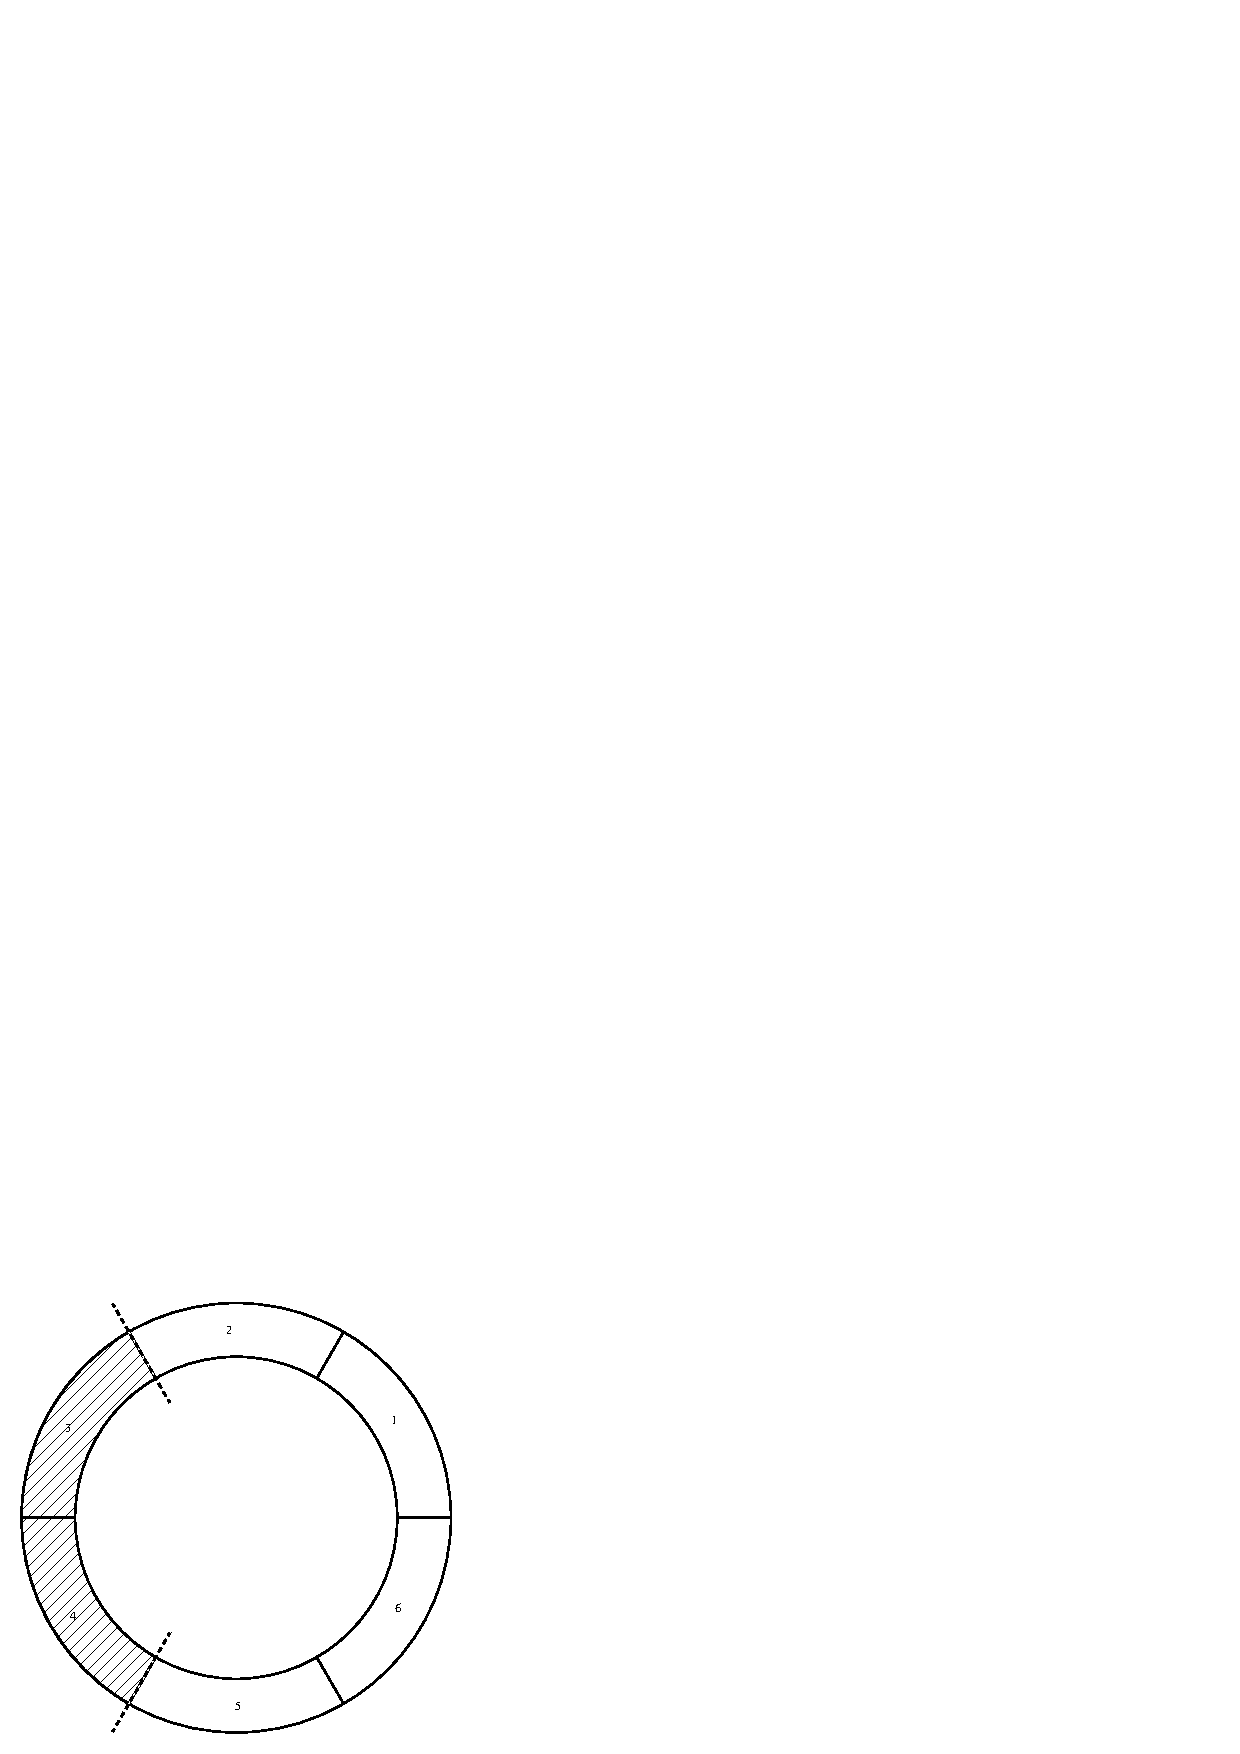
\includegraphics{fig2.pdf}
\captionof{figure}{\emph{Un parking circulaire de $6$ tirets avec une voiture garée en $(3;4)$}.}
\end{center}

Or nous remarquons immédiatement qu'une fois la voiture placée en $(3;4)$, les places adjacentes $(2;3)$ et $(4;5)$ ne sont plus disponibles (sinon les voitures se chevaucheraient et... cela n'est pas possible !). Donc, la liste des places disponibles s'est raccourcie et est devenue :
\[(1;2)\ \ \cancel{(2;3)}\ \ \cancel{(3;4)}\ \ \cancel{(4;5)}\ \ (5;6)\ \ (6;1)\]

Ainsi, il ne reste plus que $3$ places disponibles. Au hasard, supposons qu'une autre voiture se gare sur la place $(6;1)$ et nous obtenons ainsi le diagramme suivant :
\begin{center}
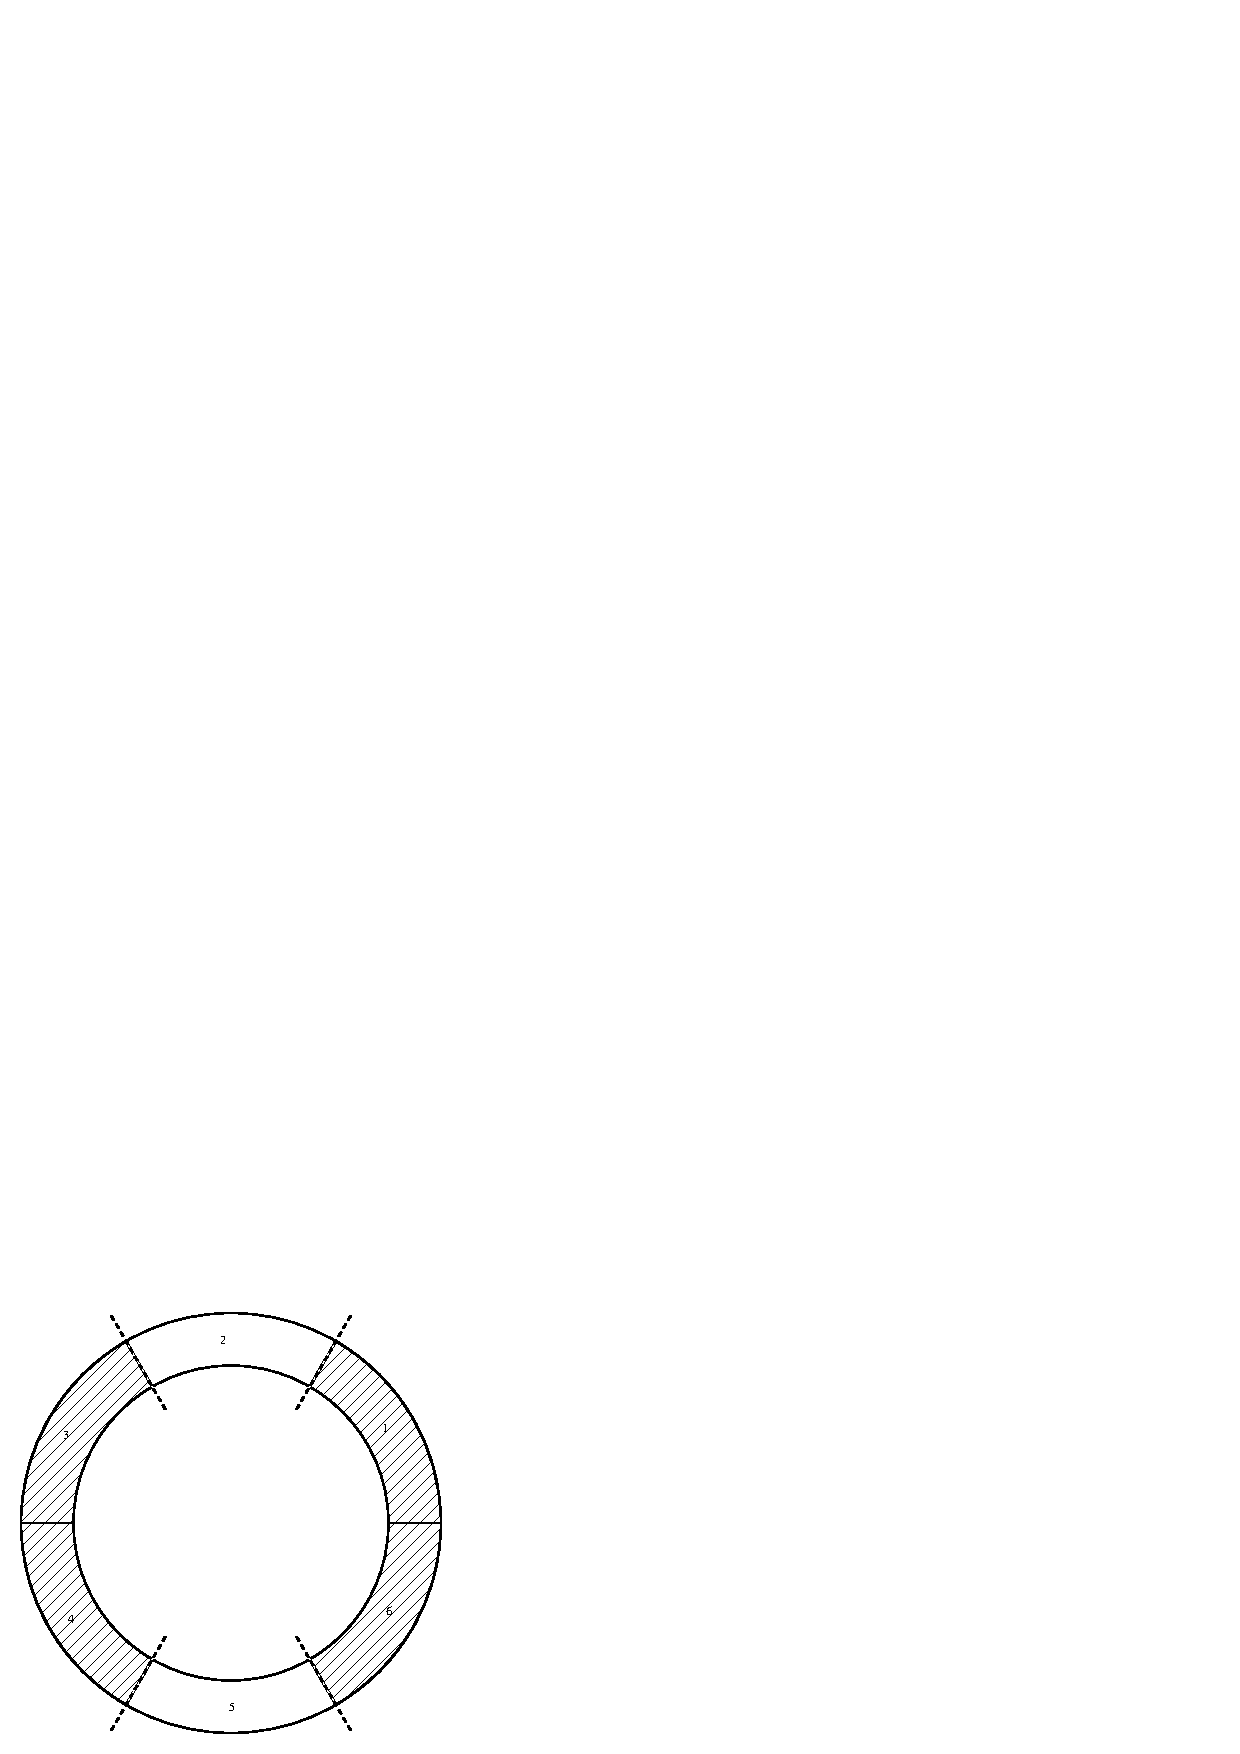
\includegraphics{fig3.pdf}
\captionof{figure}{\emph{Un parking circulaire de $6$ tirets avec une voiture garée en $(3;4)$ et en $(6;1)$}.}
\end{center}

Faisons de même avec la liste des places disponibles, nous savons que les places adjacentes à $(6;1)$ sont les places $(5;6)$ et $(1;2)$, donc supprimons-les dans notre liste des places disponibles. Nous obtenons ceci :
\[\cancel{(1;2)}\ \ \cancel{(5;6)}\ \ \cancel{(6;1)}\]

Et finalement, il ne reste aucune place disponible pour se garer (cela peut aussi se voir visuellement grâce au diagramme ci-dessus ou les tirets $2$ et $5$ ne communiquent pas). Ainsi, le nombre moyen de voitures qui se sont garées dans la situation précédente est de $2$.

Les manipulations ci-dessus sont une ébauche de l'algorithme. Elles permettent très brièvement de voir en quoi il consiste.
\subsubsection{Construction de l'algorithme}
Dans cette section nous construisons l'algorithme qui permet de placer des voitures aléatoirement sur un parking circulaire jusqu'à saturation de celui-ci. Nous obtenons :
\begin{center}
\begin{minted}[bgcolor=bg, linenos, frame=single, framesep=12pt]{text}
Construire une liste contenant toutes les places disponibles,
Tant qu'il reste des places non utilisées :
    On prend une place au hasard dans la liste,
    On supprime les places adjacentes inutilisables ainsi que celle choisie,
À la fin, on retourne le nombre total de voitures garées.
\end{minted}
\captionof{figure}{\emph{L'algorithme de placement des voitures sur un parking circulaire}.}
\end{center}

Ainsi, dans le prochain paragraphe, nous allons implémenter l'algorithme ci-dessus en Python. Mais avant cela, nous mettrons en avant les quelques erreurs à ne pas commettre lors de la mise en place du programme (nous les avons bien évidemment rencontrées).
\subsection{Mise en place du programme en Python}
Dans cette section nous implémenterons en Python l'algorithme précédemment construit. D'abord, nous listerons un ensemble de problèmes (qui ont été plus ou moins rencontrés lors de l'implémentation de l'algorithme) à ne pas commettre lors de la programmation en Python.
\subsubsection{Les erreurs d'implémentation}
Dans cette partie nous analysons les divers problèmes rencontrés lors de la conception du programme et comment ils ont été résolus.

Le premier problème rencontré a été de dire à l'ordinateur de choisir les places adjacentes à celle choisie. En effet, si celui-ci prend la $n^{ème}$ place il doit aussi prendre les $\left(n-1\right)^{ème}$ et $\left(n+1\right)^{ème}$ places. Mais le problème ne survient pas lorsque $n$ est situé au milieu de la liste mais apparaît lorsque $n=0$ ou alors que $n$ est le dernier élément de la liste.

Heureusement Python a un atout, en effet le $\left(-1\right)^{ème}$ élément de la liste désigne le dernier élément de celle-ci donc lorsque $n=0$ nous n'avons aucun problème. Mais lorsque $n$ est le dernier élément de la liste, une erreur apparaît car la $\left(n+1\right)^{ème}$ place n'existe pas. Pour y parvenir nous avons utilisé l'opérateur \emph{modulo} (notée $\%$ en Python) qui permet d'obtenir le reste de la division euclidienne par un nombre. Puisque les listes sont indexés à partir de $0$, lorsque la $n^{ème}$ place est le dernière élément de la liste alors : $n+1\pmod{ \operatorname{len}\left(liste\right)}=0$ autrement dit, on prend le $1^{er}$ élément de la liste ! Notez que la fonction $\operatorname{len}\left(liste\right)$ retourne le nombre d'éléments de la liste \emph{liste}.

Un second problème est apparut lorsque la liste ne contenait que $2$ places. En effet, l'ordinateur choisit une place au hasard mais les $2$ places adjacentes désigne le même élément. Aïe ! Pour cela, il a fallu dire à l'ordinateur que lorsqu'il n'y a que $2$ places, il ne faut prendre qu'un seul couple adjacent en utilisant une boucle $if$ qui teste si il ne reste que $2$ places.

Mais ceci a entraîné une nouvelle erreur. En effet, imaginons une liste contenant $n$ places, et supposons qu'il ne reste que deux places (particulières) comme ci-dessous :
\[[(1;2),(n;1)]\]

Le problème est que l'ordinateur comptera ces $2$ places pour $2$ positions distinctes ! Alors qu'elles représentes $3$ tirets côtes-à-côtes donc $1$ seule place disponible. Ici, il a fallu tester si, lorsqu'il ne reste que $2$ places, les deux couples adjacents représentent $2$ places distinctes (soit $4$ tirets) ou seulement $3$ tirets côtes-à-côtes ($1$ seule place disponible).
\subsubsection{Le programme Python}
Dans cette partie nous donnerons le code source du programme Python permettant la mise en œuvre de l'algorithme par la machine. Ainsi, voici le code source du programme en Python :
\begin{center}
\begin{minted}[bgcolor=bg, linenos, frame=single, framesep=12pt]{python}
from random import randint

g=lambda a:a!='' # Fonction de comparaison (voir 'filter')
n=int(input('Nb tirets: '))
l=[(i,i+1) for i in range(1,n)] + [(n,1)]

def placement():
    # On effectue une copie des places, on stocke le nombre de voitures.
    liste,voiture=l[:],0
    while liste!=[]:                   # Tant que la liste n'est pas vide.
        r=randint(0,len(liste)-1)      # On choisi un nombre aléatoire.
        voiture+=1                     # On ajoute une voiture dans la liste.
        c1,c2=(r+1)%len(liste),r-1     # On prend les places adjacentes.
        # On remplace les positions inutilisables par du vide.
        if liste[c1][0]==liste[r][1]:liste[c1]='' 
        if liste[c2]!='' and liste[c2][1]==liste[r][0]:liste[c2]=''      
        liste[r]=''                                     
        liste=list(filter(g,liste)) # On supprime les places inutilisables.
    return voiture
print(placement())
\end{minted}
\captionof{figure}{\emph{Le code source du programme Python}.}
\end{center}

Analysons un peu le programme Python ci-dessus. La ligne $1$ va de paire avec la ligne $19$ qui servent à supprimer les places inutilisables qui ont été remplacées par du vide au niveau des lignes $11$, $12$, $13$ et $14$ (et ceux, pour ne pas avoir de problème au niveau des indexes).

À la ligne $4$ on demande à l'utilisateur de choisir un nombre de tirets et en-dessous (ligne $5$) on crée la liste contenant toutes les places disponibles.

Finalement, on définit une fonction nommée \emph{placement} en ligne $7$. Nous l'appelons en ligne $21$ pour afficher le résultat. Cette fonction renvoie donc un entier qui est le nombre de voitures garées (voir la ligne $20$).

Finalement, nous avons fait fonctionner notre programme pour un nombre de tirets d'abord constant puis nous l'avons augmenté petit à petit. À chaque itération nous avons sommé le nombre moyen de voitures garées (pour un nombre de tirets constant) puis à la fin, nous avons fait une moyenne (la somme totale obtenue divisée par le nombre d'itérations effectuées). Ces résultats seront donnés dans le paragraphe suivant.
\subsection{Résultats obtenus}
Dans le paragraphe qui suit, nous présentons dans un tableau les quelques résultats obtenus avec le programme ci-dessus pour un nombre d'itérations croissant (le temps de calcul derrière a été plus ou moins long mais il ne sera pas exposé ici\footnote{Voir la partie \textbf{2.3.3
Performances : comparaison des deux formules de récurrences}.}). Ensuite nous synthétisons nos résultats sous forme d'une moyenne afin d'approximer au maximum le réel recherché : $\lambda$.

Tout d'abord, voici le tableau des résultats obtenus :
\begin{center}
\begin{tabular}{|c||c|c|}
    \hline
    \multicolumn{2}{|c|}{\textbf{Tableau des résultats obtenus}} \\ \hline\hline
        \multirow{1}{*}{\emph{Nombre d'itérations (répétitions)}} & \emph{Valeur obtenue (nombre moyen de voitures)} \\ \hline\hline
        \multirow{1}{*}{$1$} & $1743$ \\ \hline
        \multirow{1}{*}{$5$} & $1742{,}2$ \\ \hline
        \multirow{1}{*}{$10$} & $1742{,}3$ \\ \hline
        \multirow{1}{*}{$50$} & $1738{,}93$ \\ \hline
        \multirow{1}{*}{$100$} & $1740{,}6$\\ \hline
        \multirow{1}{*}{$500$} & $1740{,}694$ \\ \hline
        \multirow{1}{*}{$1000$} & $1740{,}335$ \\
    \hline
\end{tabular}
\captionof{figure}{\emph{Tableau du nombre moyen de voitures pour un nombre d'itérations croissant}.}
\end{center}

Ainsi, comme nous le montre l'approche numérique par un programme, le nombre moyen de voitures qui se garent sur $4026$ tirets doit être relativement proche de $1740$. Ainsi on peut dire que :
\[\lambda \approx 1740\]

Mais afin d'obtenir un résultat (peut-être) meilleur, il faut effectuer une moyenne pondérée avec les résultats du tableau ci-dessus. Donc, nous avons la moyenne pondérée suivante :
\[\lambda\approx\frac{1}{1666}\left(1743+5\times1735{,}4+\ldots+1000\times1740{,}335\right)\approx1740{,}4354741\]

Notez que l'approximation ci-dessus contient $2$ décimales exactes pour seulement $1666$ itérations ! Ainsi, nous pouvons remarquer que l'usage de l'outil informatique peut être efficace notamment pour d'accélérer le cadrage des conjectures (et notamment de vérifier la cohérence de la solution théorique). En effet, nous obtenons, aux vues des les résultats ci-dessus, une très bonne approximation de $\lambda$.

Nous pouvons aussi calculer la part de cette approximation par rapport au nombre total de tirets présents dans le parking ? Ainsi nous obtenons :
\[\frac{\lambda}{4026}\approx\frac{1740{,}4354741}{4026}\approx0{,}43229892550919025\]

Ainsi, nous pouvons déjà prédire (à peut près) sans outil théorique que la solution, $\lambda$, avoisinera les $43\%$ de $4026$.
\subsection{Avantages \& inconvénients de l'outil informatique}
L'outil informatique a de nombreux avantages dans les problèmes liés, surtout, à la simulation comme celui des voitures qui se garent par exemple. Mais sa puissance réside avant tout dans le fait qu'il peut effectuer un grand nombre de calculs tout en gardant une précision raisonnable (une dizaine de décimales tout au plus par défaut).

Ainsi, nous pouvons remarquer que l'approche numérique a permis de résoudre partiellement le problème en approximant le réel recherché : $\lambda$. En effet nous sommes partis du fait que :
\[\lambda\in\left[1342;2013\right]\]

Avant d'arriver à la conclusion que :
\[\lambda\approx1740{,}4354741\]

Ce qui constitue une énorme avancée depuis le début du problème. Mais chaque outil à ses inconvénients. En effet, nous avons remarqué que pour simuler l'expérience sur un grand nombre d'itérations, le temps de calcul était de plus en plus long (plus de $2$ minutes pour $1000$ itérations !). 

De plus, la simulation sur un très grand nombre d'itérations conduit parfois à des erreurs liées aux décimales (même minimes et peu significatives pour $n=4026$ mais dramatiques pour un nombre de tirets de plus en plus grand). 

De même, bien que l'approche numérique soit un bon outil pour montrer un résultat, ce n'est pas une preuve formelle ! Ainsi, rien ne nous garantit que : $\lambda\approx1740{,}4354741$ (car tout repose sur des probabilités) ! En effet, refaire l'expérience nous donnera un résultat différent de celui obtenu par la moyenne pondérée alors que la solution, $\lambda$, n'aura pas changée de valeur puisque c'est une \textbf{constante} !

Finalement même si l'ordinateur constitue un outil solide, il ne permet qu'au cadrage des conjectures afin de donner un point de vue de l'ordre de grandeur de la solution. C'est pourquoi nous allons utiliser une nouvelle approche plus formelle, l'approche théorique : les mathématiques\footnote{Même si l'usage des mathématiques était présente auparavant, elle n'en était pas la ligne directrice, dans la seconde section c'est elle qui domine.}.
\section{Les mathématiques - l'approche théorique}
Une fois les simulations informatiques terminées et l'approche numérique achevée, nous pouvons commencer l'approche théorique, beaucoup plus formelle, abstraite (parfois) et directe. En effet, l'algorithme mis en œuvre plus haut permet de se faire une idée de comment parvenir à la formule (par récurrence ?).

Dans un premier temps, nous mettrons en place une notation bien spécifique que nous utiliserons tout le long de cette section. Puis, nous commencerons à analyser quelques résultats préliminaires avant d'extraire la formule générale. Et finalement, nous améliorerons la formule afin d'optimiser le temps de calcul.

\subsection{Notation et essaies préliminaires}
\subsubsection{Notation}
Premièrement, nous allons nous fixer une notation bien précise afin de désigner chaque composante efficacement et rapidement. 

Puisqu'il y a deux types de parking (et donc $2$ solutions possibles) nous allons créer deux fonctions : $\operatorname{C}(t)$ qui correspond au nombre moyen de voitures qui se garent dans un parking circulaire de $t$ tirets et $\operatorname{L}(t)$ une fonction similaire mais dans un parking linéaire (de $t$ tirets aussi).

Ainsi, puisqu'il y a deux parkings différents, il y a aussi deux solutions distinctes, par convention appelons ces deux réels : $\lambda_C=\operatorname{C}(4026)$ et $\lambda_L=\operatorname{L}(4026)$ (ils correspondent au nombre moyen de voitures qui se garent dans un parking circulaire de $4026$ tirets et un parking linéaire de $4026$ tirets). Nous désignerons aussi par : $t$ le nombre total de tirets du parking et par $p_C\left(t\right)$ (respectivement $p_L\left(t\right)$) le nombre total de places dans un parking circulaire (respectivement linéaire) de $t$ tirets et chaque place sera repérée par un unique couple de coordonnées.

Ainsi, nous pouvons maintenant commencer à observer quelques relations et propriétés simples qui lient les deux fonctions et qui nous mènerons vers la formule générale de récurrence.
\subsubsection{Essaies préliminaires}
Ainsi, dans cette partie, nous allons montrer, pour des parkings avec un petit nombre de tirets, qu'il y a un schéma répétitif dans le calcul du nombre moyen de voitures qui se garent dans un parking. Ceci permettra dans le paragraphe suivant d'aboutir à la formule générale de récurrence. Mais avant cela considérons quelques calculs sur les fonctions : $\operatorname{C}\left(t\right)$ et $\operatorname{L}\left(t\right)$ qui sont résumés dans les deux tableaux ci-dessous :
\begin{center}
\begin{tabular}{|c||c|c|}
    \hline
    \multicolumn{2}{|c|}{\textbf{Tableau valeur de $\operatorname{C}\left(t\right)$}} \\ \hline\hline
        \multirow{1}{*}{\emph{Nombre de tirets - $t$}} & \emph{Nombre moyen de voitures} \\ \hline\hline
        \multirow{1}{*}{$0$} & $0$ \\ \hline
        \multirow{1}{*}{$1$} & $0$ \\ \hline
        \multirow{1}{*}{$2$} & $1$ \\ \hline
        \multirow{1}{*}{$3$} & $1$ \\ \hline
        \multirow{1}{*}{$4$} & $2$\\ \hline
        \multirow{1}{*}{$5$} & $2$ \\
    \hline
\end{tabular}
\captionof{figure}{\emph{Tableau de valeur de la fonction : $\operatorname{C}\left(t\right)$ avec : $0\leqslant t\leqslant 5$}.}
\end{center}

En faite, il est en réalité assez simple de calculer le nombre moyen de voitures pour un nombre $t$ de tirets relativement bas.

Or lorsque $t=6$, cela devient plus difficile et répondre mentalement au problème devient plus complexe. Ci-dessous nous synthétisons aussi les résultats (basiques) obtenus avec la seconde fonction :
\begin{center}
\begin{tabular}{|c||c|c|}
    \hline
    \multicolumn{2}{|c|}{\textbf{Tableau valeur de $\operatorname{L}\left(t\right)$}} \\ \hline\hline
        \multirow{1}{*}{\emph{Nombre de tirets - $t$}} & \emph{Nombre moyen de voitures} \\ \hline\hline
        \multirow{1}{*}{$0$} & $0$ \\ \hline
        \multirow{1}{*}{$1$} & $0$ \\ \hline
        \multirow{1}{*}{$2$} & $1$ \\ \hline
        \multirow{1}{*}{$3$} & $1$ \\
    \hline
\end{tabular}
\captionof{figure}{\emph{Tableau de valeur de la fonction : $\operatorname{L}\left(t\right)$ avec : $0\leqslant t\leqslant 3$}.}
\end{center}

Ici aussi, à partir d'un nombre de tirets, $t$, supérieur à $4$ le calcul mental laisse place au papier et au crayon. Mais lorsque nous regardons de plus près aux $4$ première valeurs des deux tableaux nous remarquons que lorsque : $0\leqslant t \leqslant 3$ alors : $\operatorname{C}\left(t\right)=\operatorname{L}\left(t\right)$. Ainsi nous pouvons en déduire qu'il doit y avoir une relation entre ces deux fonctions. Mais laquelle ?

En regardant de plus près le nombre total de places disponibles dans un parking circulaire et dans un parking linéaire pour un même nombre de tirets nous remarquons quelque chose d'intéressant :
\[p_{C}\left(t\right)=1+p_{L}\left(t\right)\]

En effet, dans un parking linéaire les deux tirets aux extrémités ne sont pas reliés entre-eux, ce qui n'est pas le cas dans le parking circulaire donc il y a une place de plus dans un parking circulaire que dans un parking lin"aire de même nombre de tirets. 

Ainsi, la méthode pour relier les deux fonctions serait de faire en sorte que dans le parking circulaire il y ait $2$ tirets qui ne soit pas reliés entre-eux. 

Or ceci n'apparaît que lorsqu'une voiture s'est garée ! Et donc, nous obtenons notre fameuse relation entre les deux fonctions :
\[\operatorname{C}\left(t\right)=1+\operatorname{L}\left(t-2\right),\ \ \ \text{avec : $t\geqslant 2$}\]

Nous pouvons aussi trouver cette relation grâce aux diagrammes. Par exemple, prenons un parking circulaire de $6$ tirets. Voici le diagramme que nous obtenons :
\begin{center}
\includegraphics{fig4.pdf}
\captionof{figure}{\emph{Un parking circulaire de $6$ tirets}.}
\end{center}

Maintenant, supposons qu'une voiture se place, au hasard, en $(1;2)$. De ce fait, nous obtenons le nouveau diagramme suivant :
\begin{center}
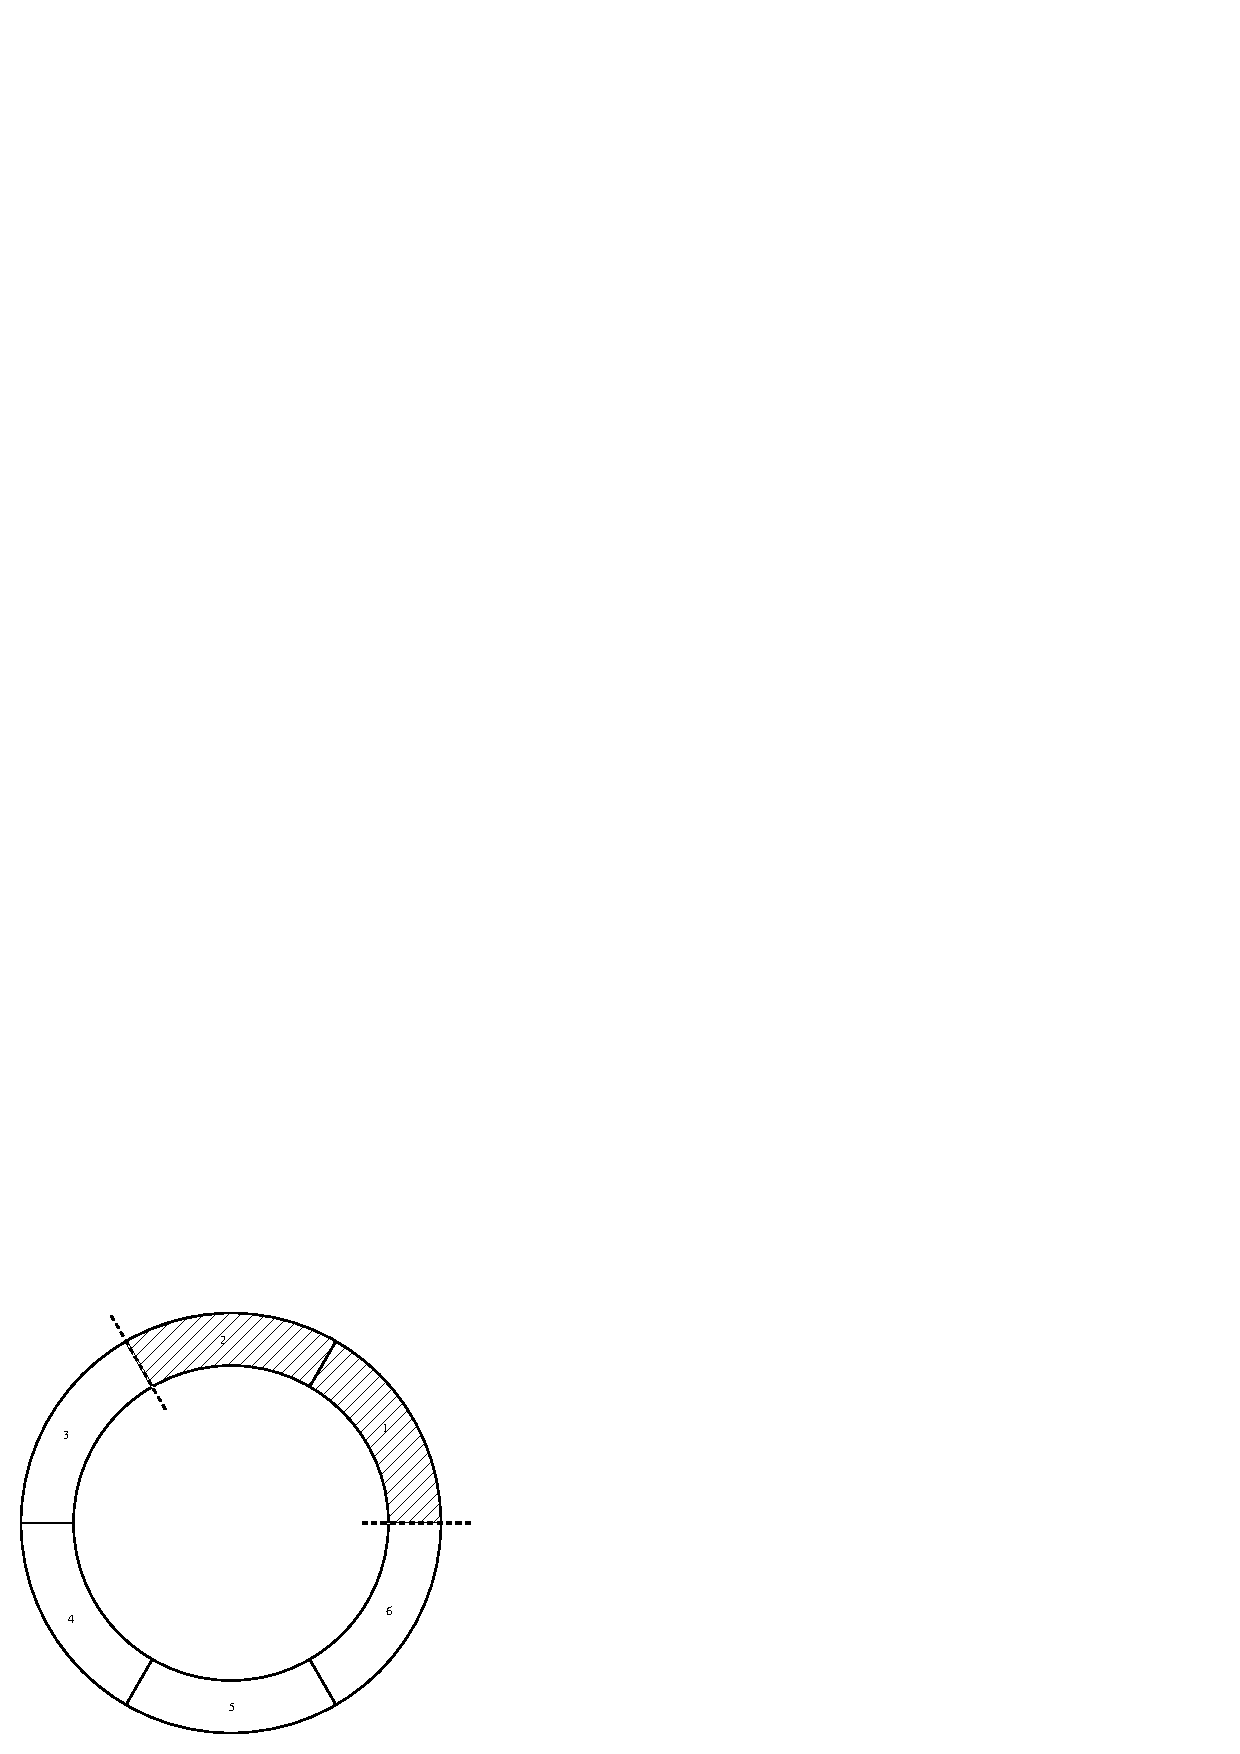
\includegraphics{fig5.pdf}
\captionof{figure}{\emph{Un parking circulaire de $6$ tirets avec une voiture garée en $(1;2)$}.}
\end{center}

Et nous pouvons alors remarquer que les tirets $3$ et $6$ ne communiquent plus directement, ils ne sont plus liés entre-eux. Autrement dit, la voiture qui vient de se garer agit comme une barrière. Et ainsi, en dépliant le parking par rapport à l'une des extrémités de la voiture positionnée nous obtenons le parking suivant :
\begin{center}
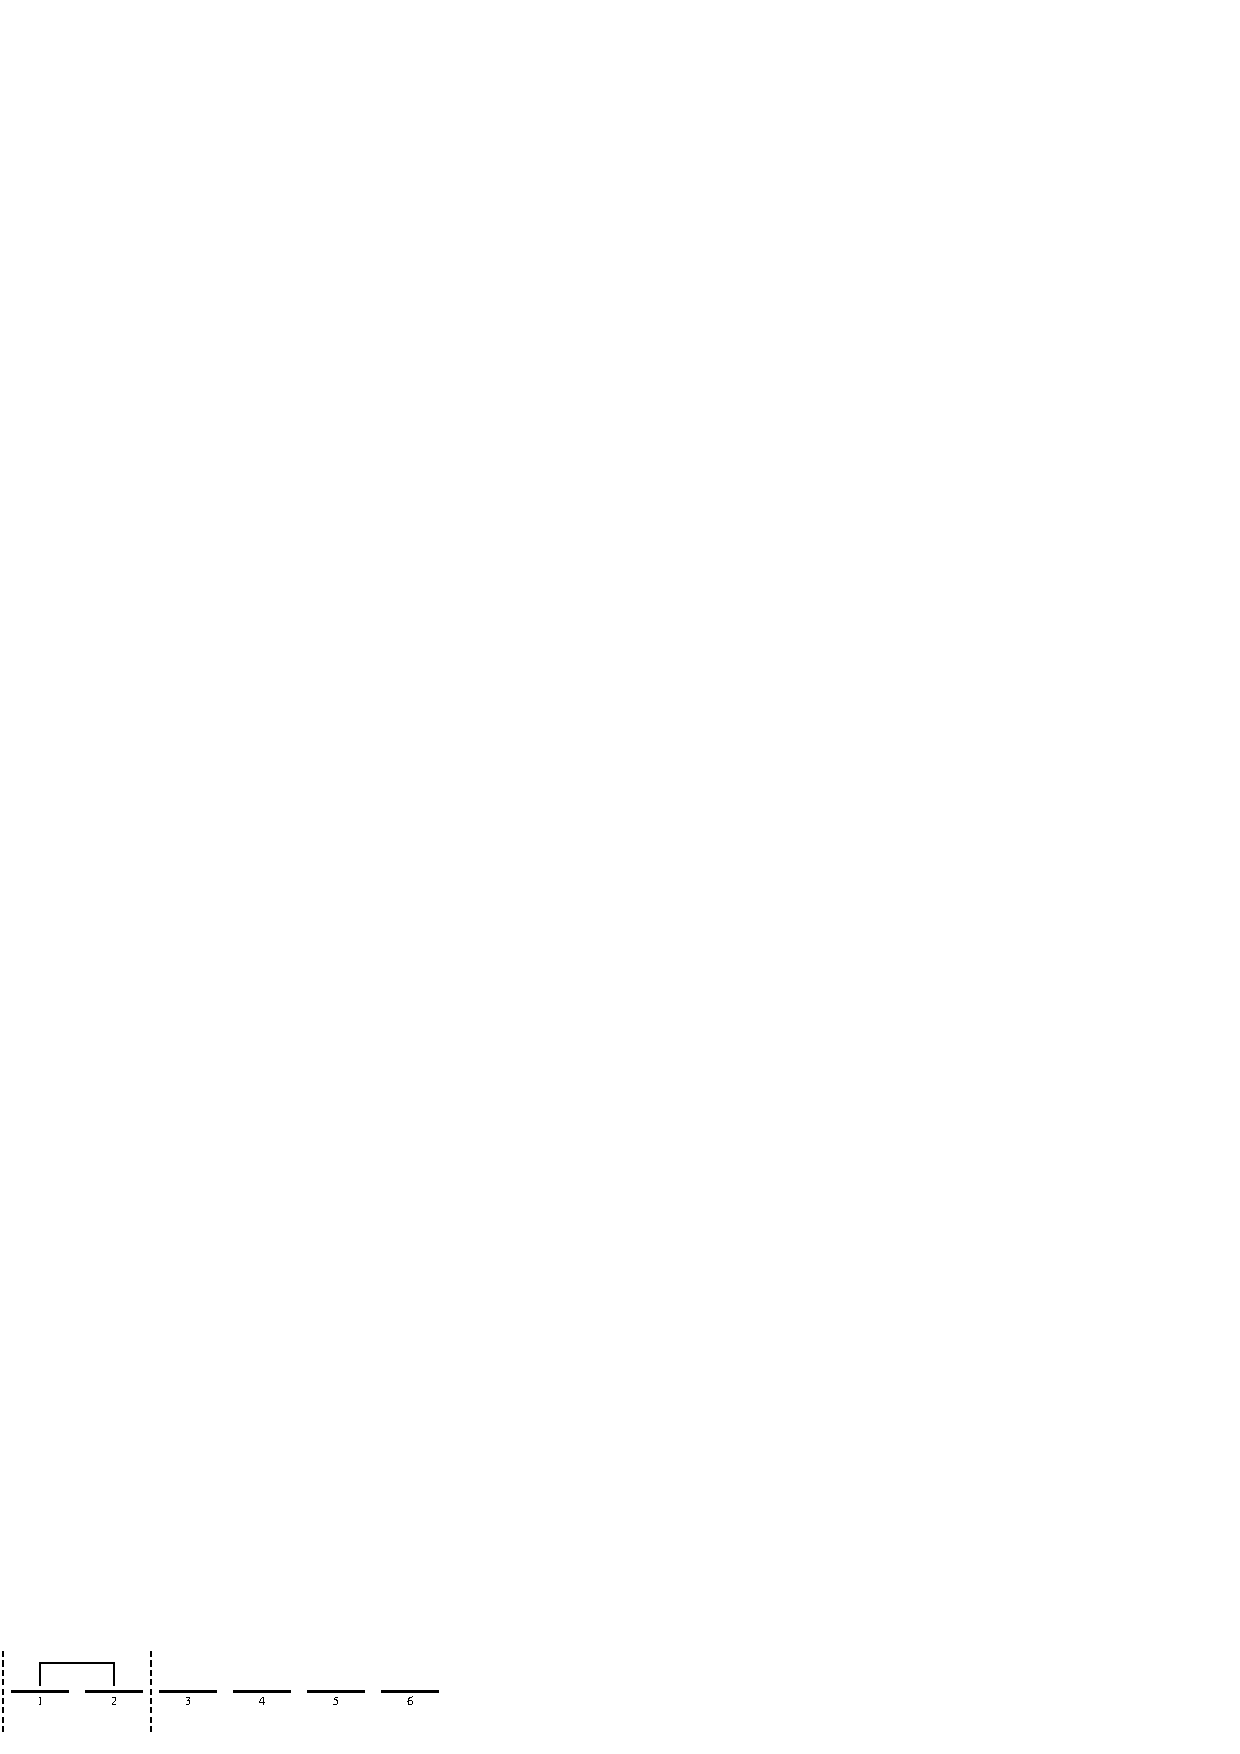
\includegraphics{fig6.pdf}
\captionof{figure}{\emph{Un parking linéaire de $6$ tirets avec une voiture garée en $(1;2)$}.}
\end{center}

Et nous pouvons correctement voir qu'il ne reste plus que $4$ tirets au lieu de $6$. Et de manière générale, puisqu'une voiture prend $2$ tirets, cela prouve bien que la relation entre : $\operatorname{C}\left(t\right)$ et $\operatorname{L}\left(t\right)$ est vraie.

Ainsi, maintenant que la relation entre parking circulaire et linéaire a été établie, nous ne travaillerons désormais plus qu'avec des parkings linéaires dans la suite du sujet. 

Nous allons maintenant trouver une manière de calculer le nombre moyen de voitures qui se garent. Pour cela, il faut repérer un schéma générale afin de l'extraire et finalement, trouver la formule de récurrence.
\subsection{La formule de récurrence}
Dans ce paragraphe, nous allons vous présenter toutes les formules que nous avons obtenus et qui permettent de calculer le nombre moyen de voitures qui se garent sur un parking (linéaire) afin de finalement résoudre le problème en trouvant les solutions $\lambda_L$ et $\lambda_C$.

Dans un premier temps, nous allons nous concentrer sur des parkings linéaires avec un nombre, $t$, de tirets inférieur à $6$. Nous utiliserons les arbres pondérés avant de formaliser définitivement la formule. Finalement, nous l'améliorerons afin de l'optimiser pour les calculs informatiques.
\subsubsection{La formule \emph{brute}}
Dans cette partie, nous allons mettre en place une technique récursive permettant de calculer le nombre moyen de voitures qui se garent sur un parking linéaire. Puis nous montrerons la formule que nous avons trouvée.

Premièrement, prenons un parking linéaire constitué de deux tirets. Il est assez simple de voir que le nombre moyen de voitures garées est de $1$ puisqu'il n'y a qu'une seule place disponible :
\begin{center}
\includegraphics{fig7.pdf}
\captionof{figure}{\emph{Un parking linéaire de $2$ tirets avec une voiture garée en $(1;2)$}.}
\end{center}

Mais maintenant, si, au lieu de prendre $2$ tirets nous en prenions $3$. Malgré tout, le nombre moyen de voitures garées reste toujours de $1$. En effet nous avons le choix entre deux places différentes : soit la place $(1;2)$, soit $(2;3)$ :
\begin{center}
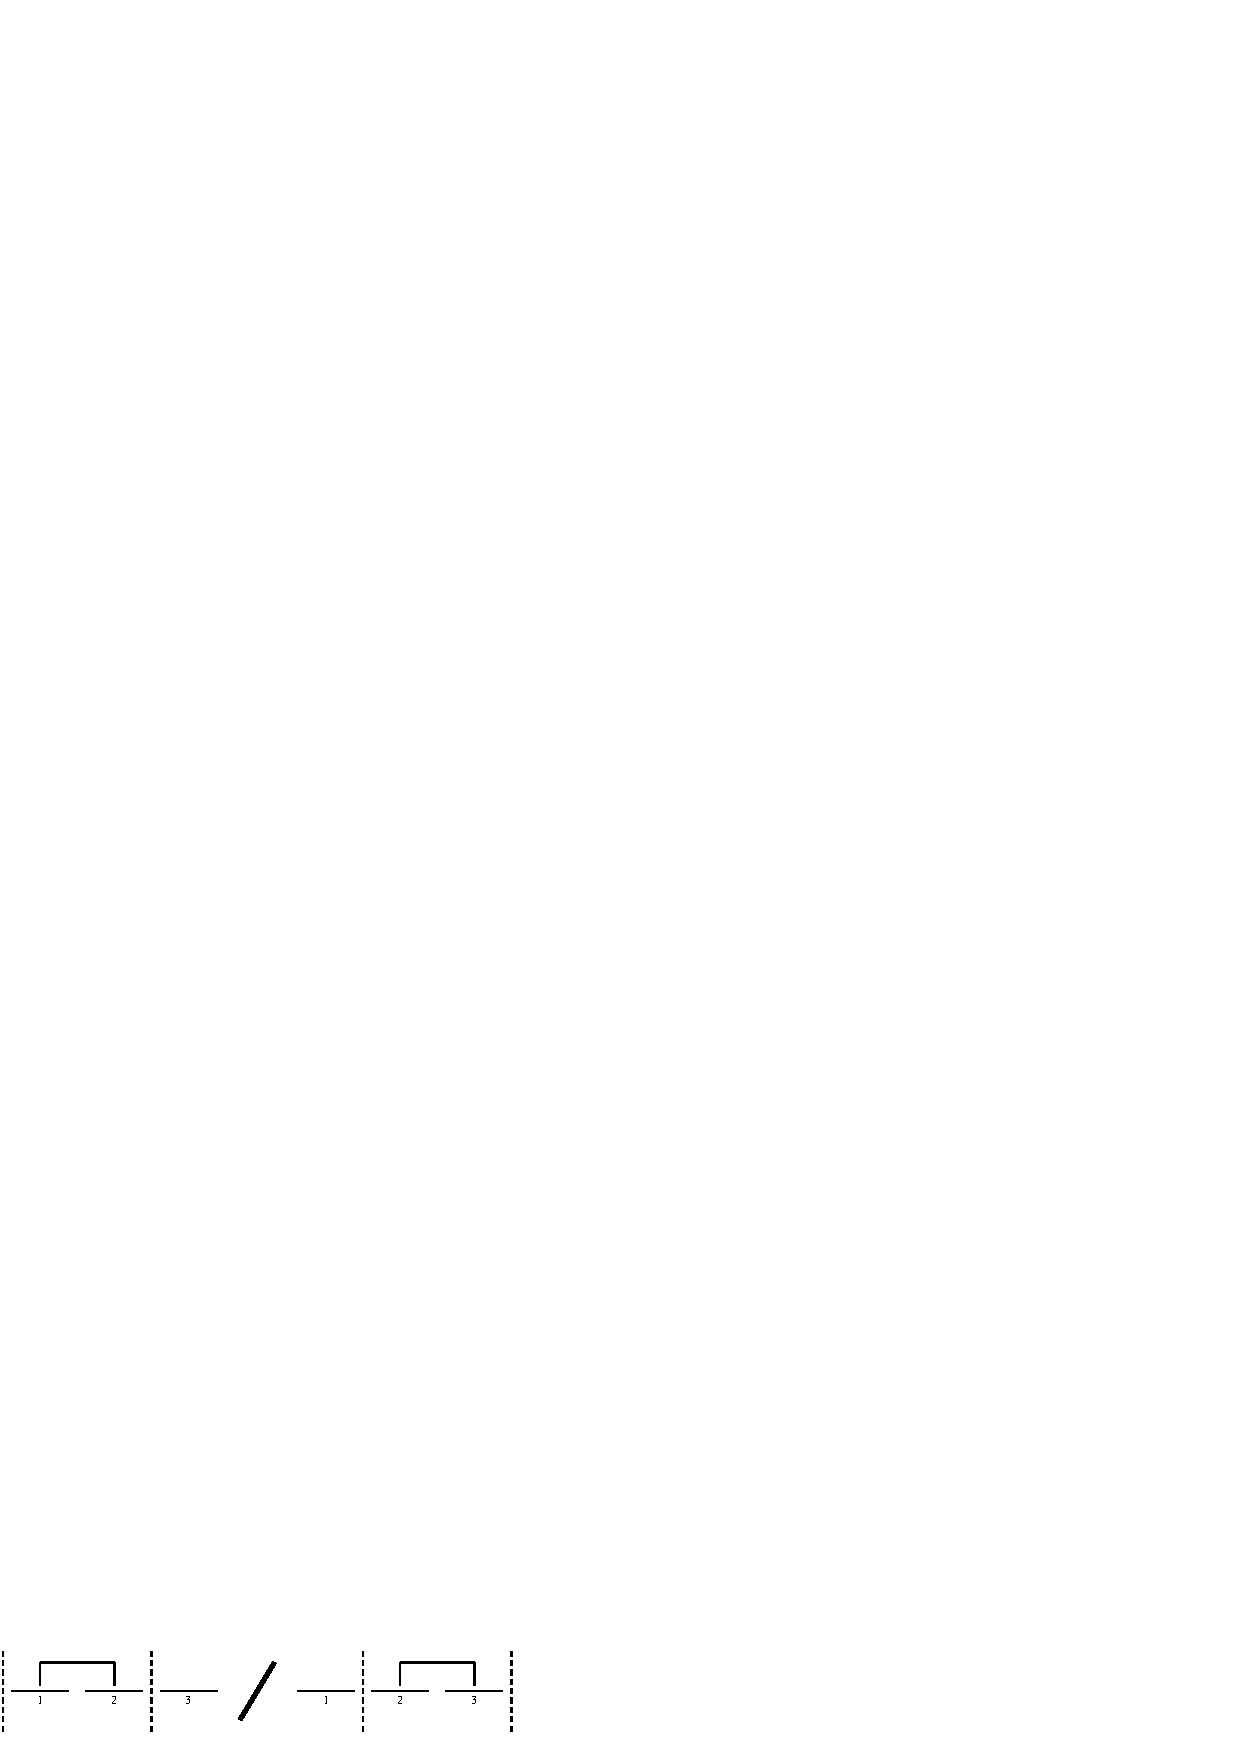
\includegraphics{fig8.pdf}
\captionof{figure}{\emph{Deux parkings linéaires de $3$ tirets avec une voiture garée en $(1;2)$ et en $(2;3)$}.}
\end{center}

En faite il est assez simple de remarquer que lorsque la première voiture se gare, il ne reste que $1$ tiret vide, donc, il n'y a plus de places disponibles. Mais pour un parking linéaire de $4$ tirets, la chose est plus complexe. En effet, nous avons le parking suivant :
\begin{center}
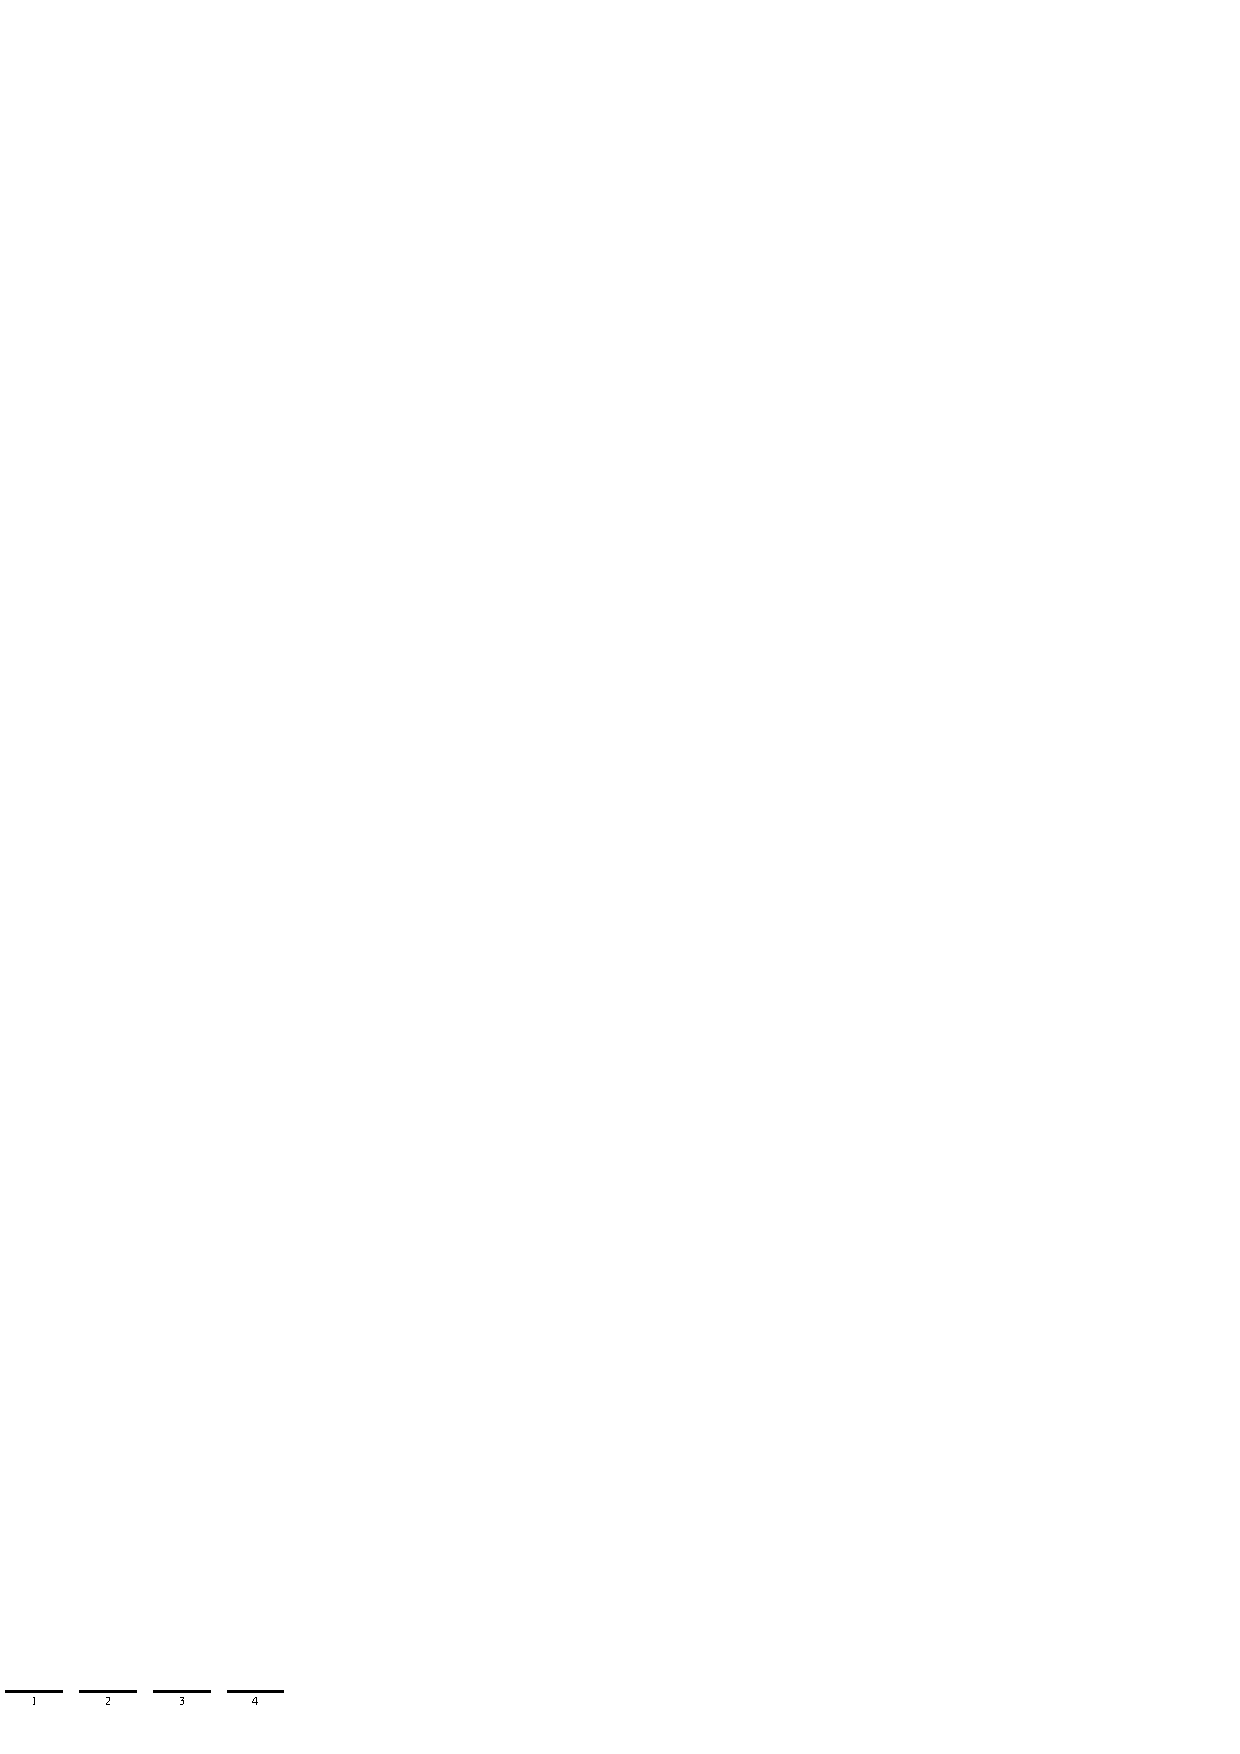
\includegraphics{fig9.pdf}
\captionof{figure}{\emph{Un parking linéaire de $4$ tirets}.}
\end{center}

Or, nous remarquons une chose intéressant. Nous savons qu'au total, il y a $3$ places disponibles : $(1;2)$, $(2;3)$ et $(3;4)$. Mais, lorsqu'une voiture se gare, au hasard, sur les cases: $(1;2)$ ou $(3;4)$, alors, le nombre total de voitures garés sera forcément de $2$ puisque le parking sera saturé. 

De même lorsqu'une voiture se gare au centre (sur la place $(2;3)$), alors, le nombre total de voitures garées est seulement de $1$, comme le montre les deux diagrammes suivants (les flèches symbolisent que la voiture suivante se garera automatiquement à côté de celle déjà placée) :
\begin{center}
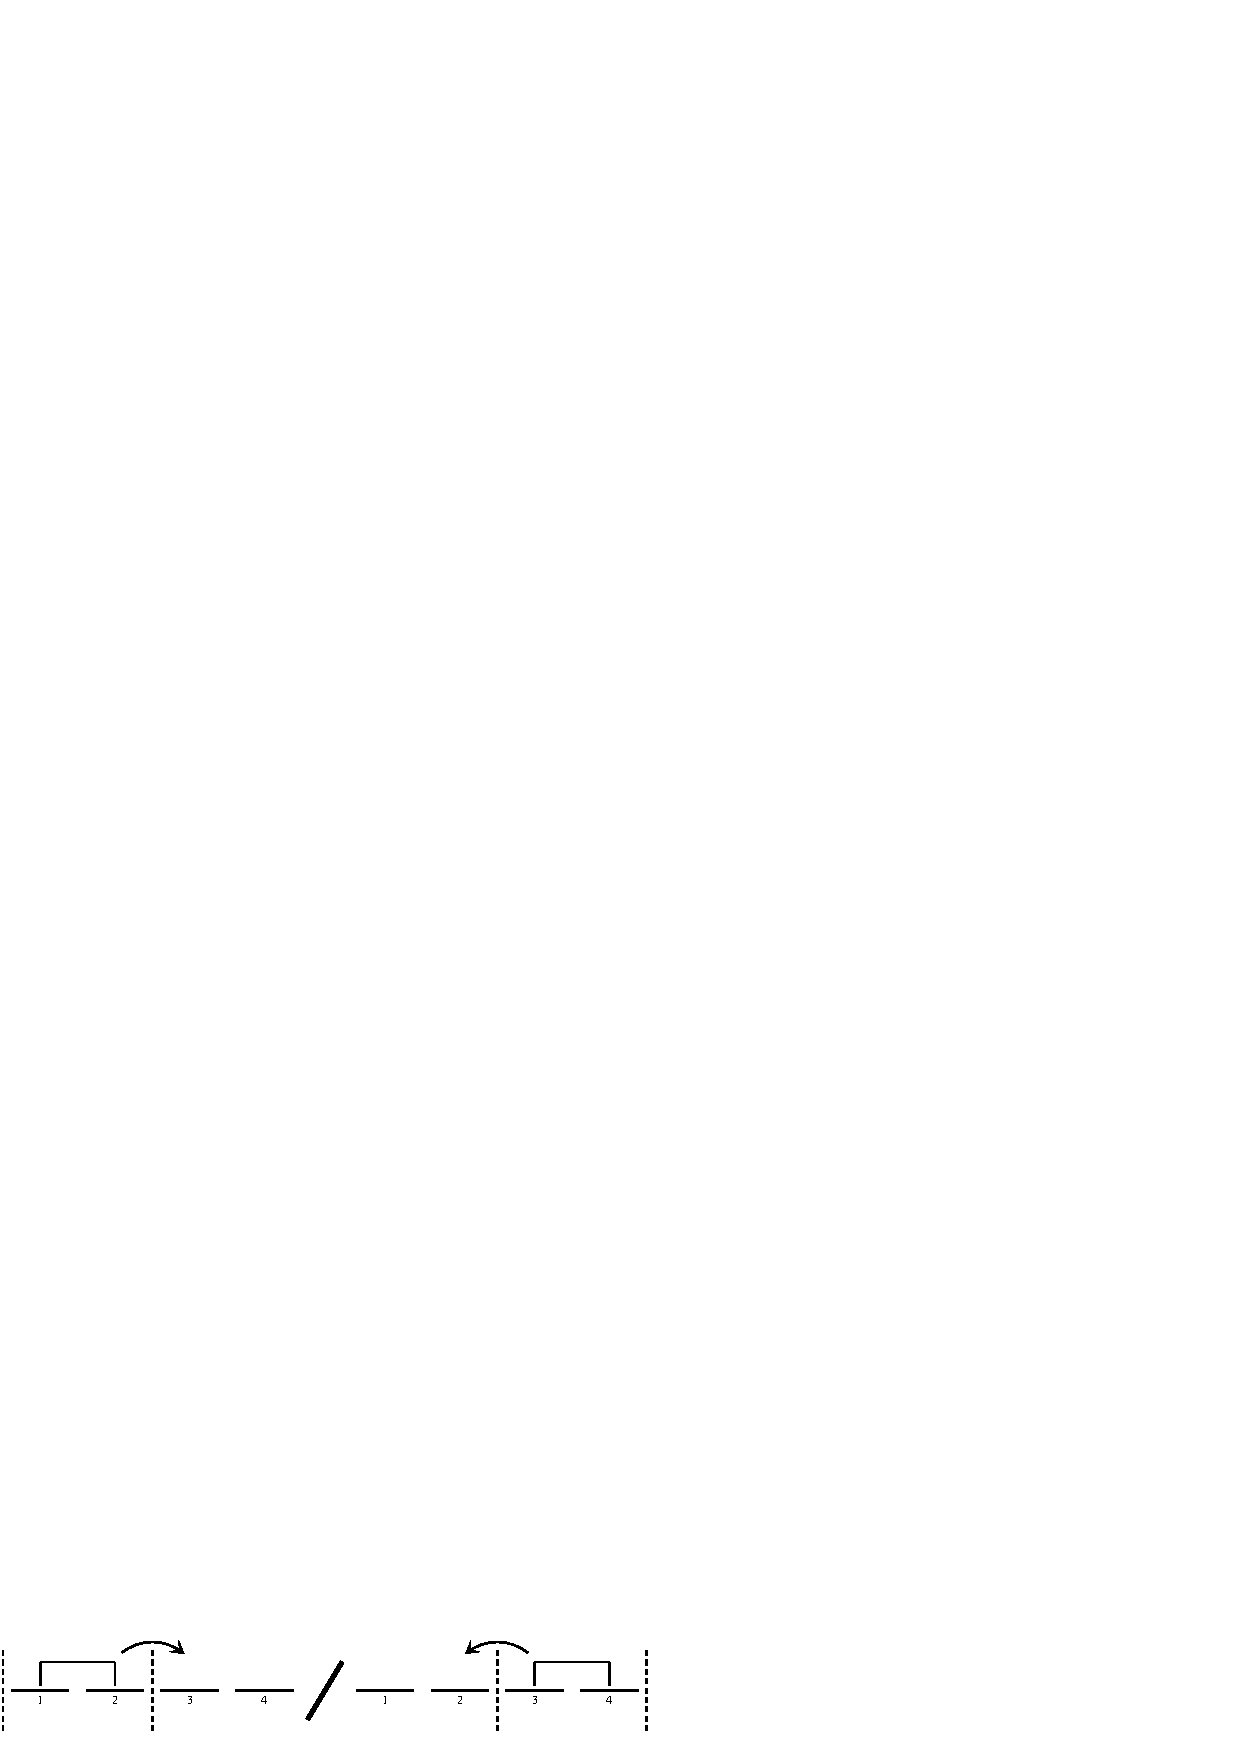
\includegraphics{fig10.pdf}
\captionof{figure}{\emph{Deux parkings linéaires de $4$ tirets avec une voiture garée en $(1;2)$ et en $(3;4)$}.}
\end{center}

Et finalement, il ne nous reste que la place centrale à utiliser (de coordonnées : $(2;3)$), ainsi, voici le diagramme obtenu:
\begin{center}
\includegraphics{fig11.pdf}
\captionof{figure}{\emph{Un parking linéaire de $4$ tirets avec une voiture garée en : $(2;3)$}.}
\end{center}

Ainsi, dans le cas ci-dessus, nous avons une seule voiture garée. Donc, comme nous l'avons signalé précédemment, nous pouvons résumer tous ceci dans un arbre pondéré des possibles comme ci-dessous :
\begin{center}
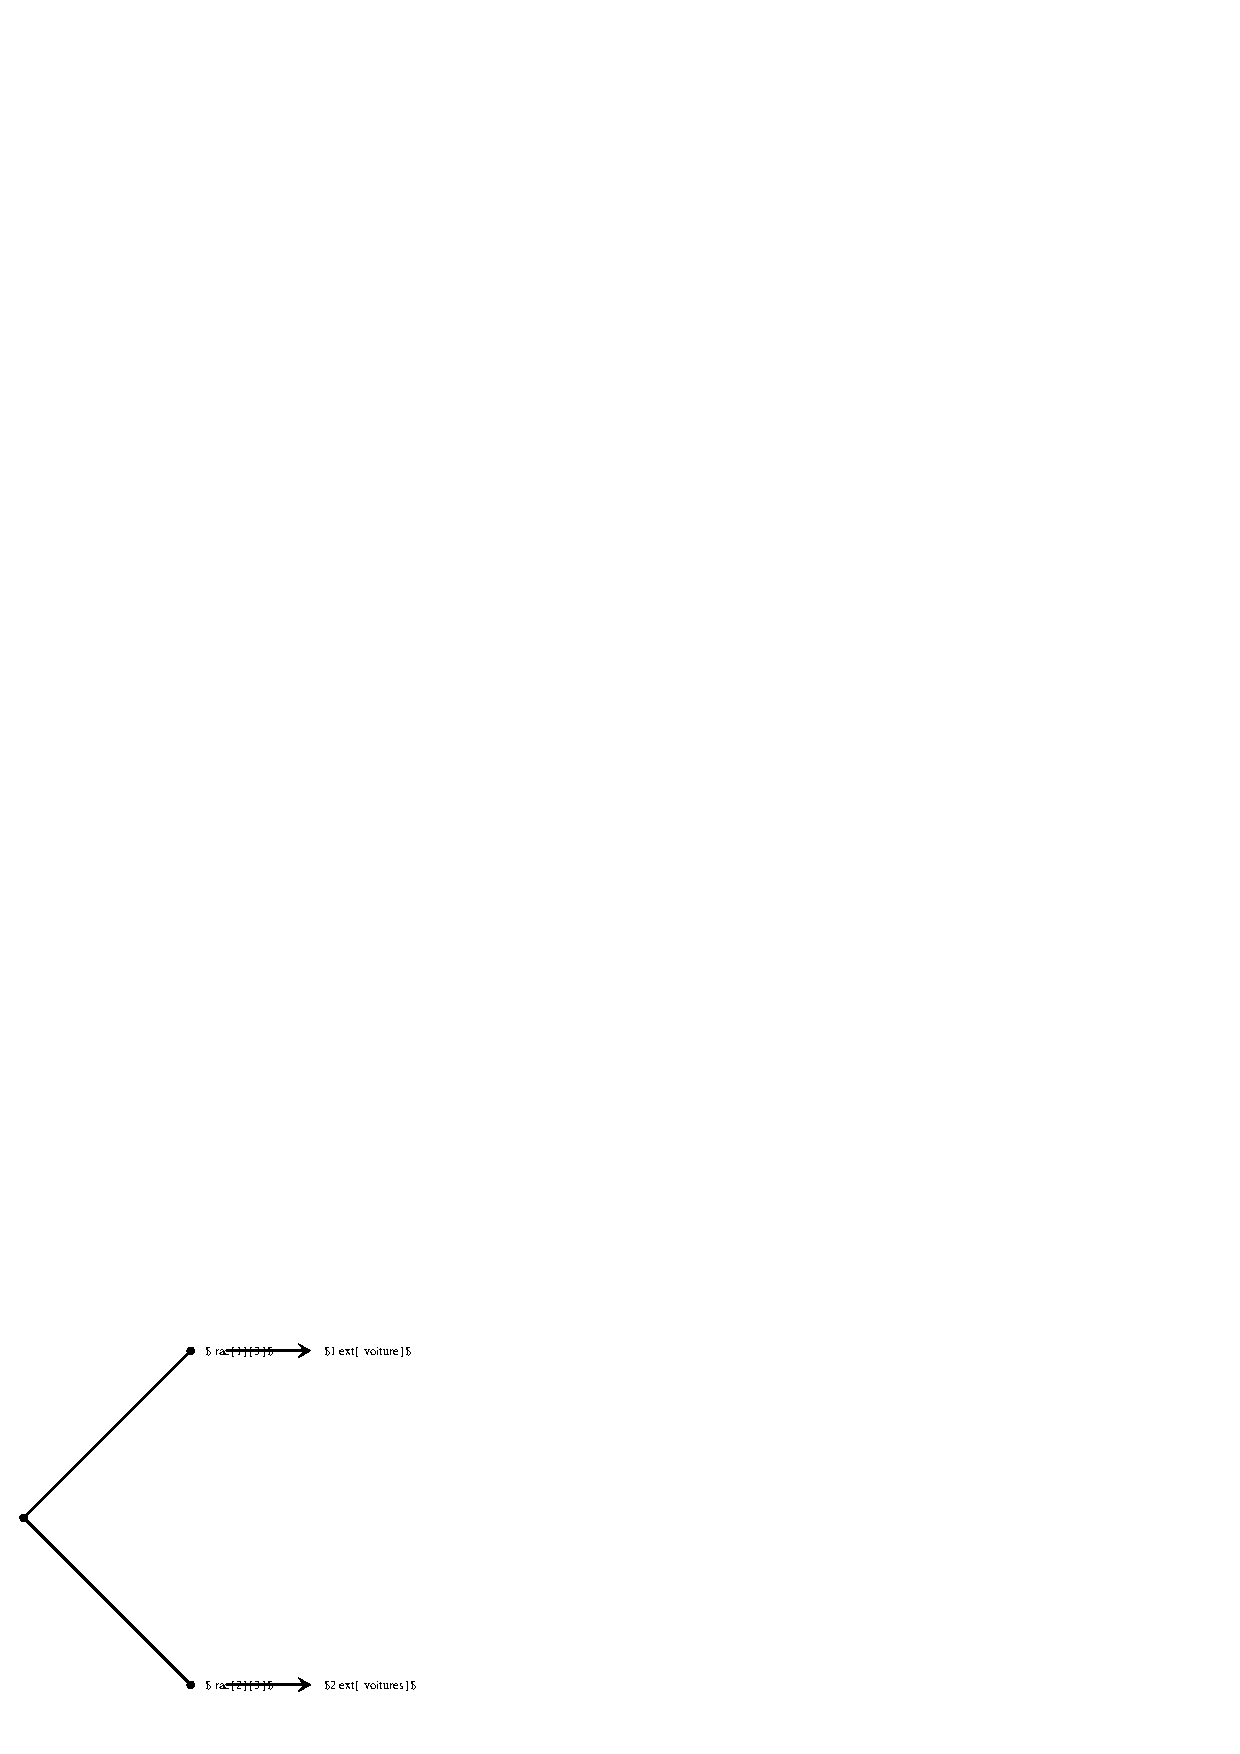
\includegraphics{fig12.pdf}
\captionof{figure}{\emph{L'arbre pondéré des possibles pour un parking linéaire de $4$ tirets}.}
\end{center}

Et finalement, en faisant la moyenne de l'arbre pondéré ci-dessus nous obtenons :
\[\operatorname{L}\left(4\right)=2\times\frac{2}{3}+1\times\frac{1}{3}=\frac{\left(2\times2\right)+\left(1\times1\right)}{3}=\frac{5}{3}\approx1{,}666667\]

Et donc, nous avons finalement répondu à la question que nous nous étions posée. Il découle que le nombre moyen de voitures qui se garent sur un parking linéaire de $4$ tirets et de $\frac{5}{3}$. 

Mais quand est-il pour un parking linéaire de $5$ tirets ? Eh bien, la réponde est assez simple puisque: $\operatorname{L}\left(5\right)=2$. En effet, lorsque la voiture se gare sur la place : $(1;2)$, une seconde peut aussi se garer sur les $3$ places manquantes. De même, si une voiture se gare sur la place $(2;3)$, il reste $2$ places à droite. Et finalement, on finit par la symétrie (les voitures se gareront du côté gauche plutôt que celui de droit).

Mais en continuant, qu'en est-il de : $\operatorname{L}\left(6\right)$ ? C'est à partir d'ici que vas commencer à apparaître la formule de récurrence.

Dans un premier temps, prenons un parking linéaire composé de $6$ tirets comme ci-dessous:
\begin{center}
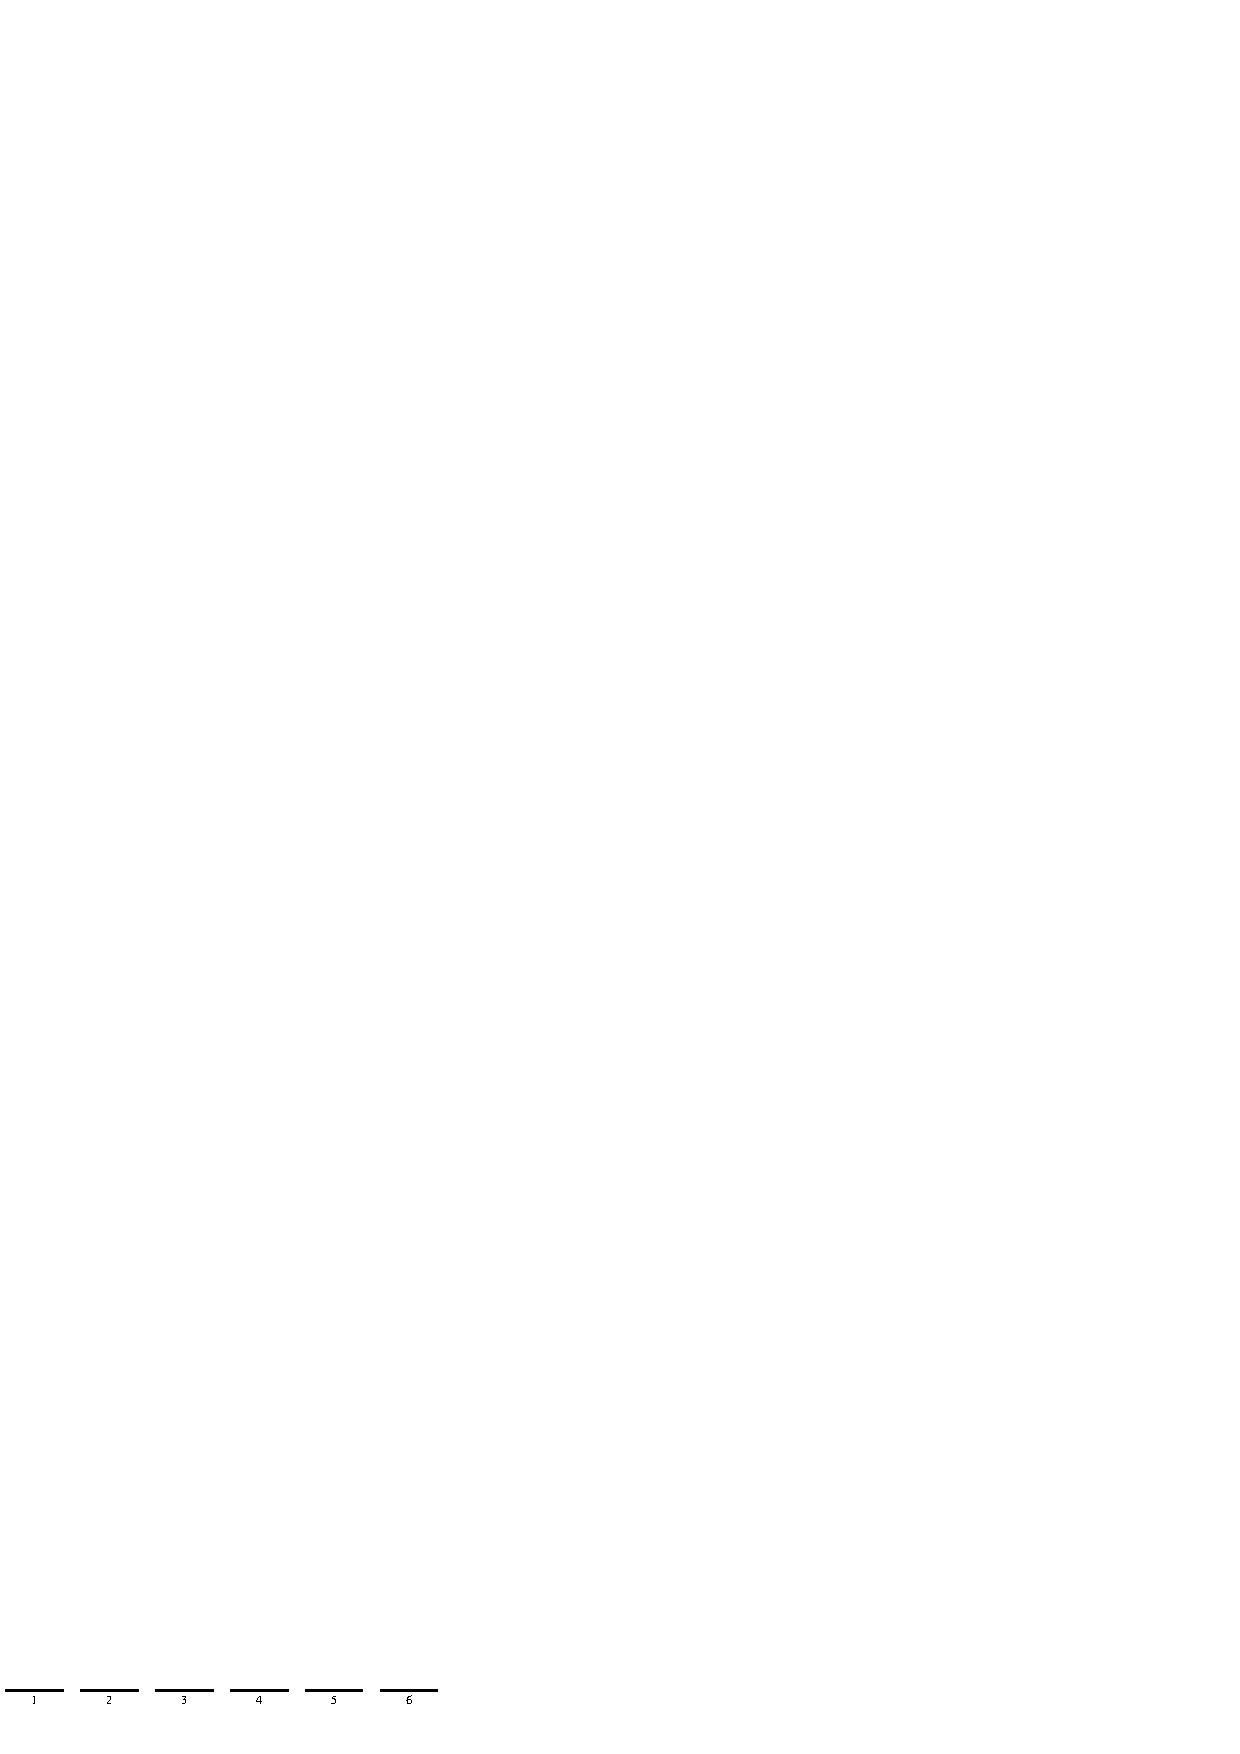
\includegraphics{fig13.pdf}
\captionof{figure}{\emph{Un parking linéaire de $6$ tirets}.}
\end{center}

Nous savons que ce parking est constitué de $5$ places distinctes. Ainsi, il y a $1$ chance sur $5$ que la première voiture se gare à la place $(1;2)$. De même pour la place $(2;3)$ et ainsi de suite... Donc, nous pouvons découper notre parking en $5$ autres parkings (que nous appellerons symboliquement \emph{sous-parkings}) que voici :
\begin{center}
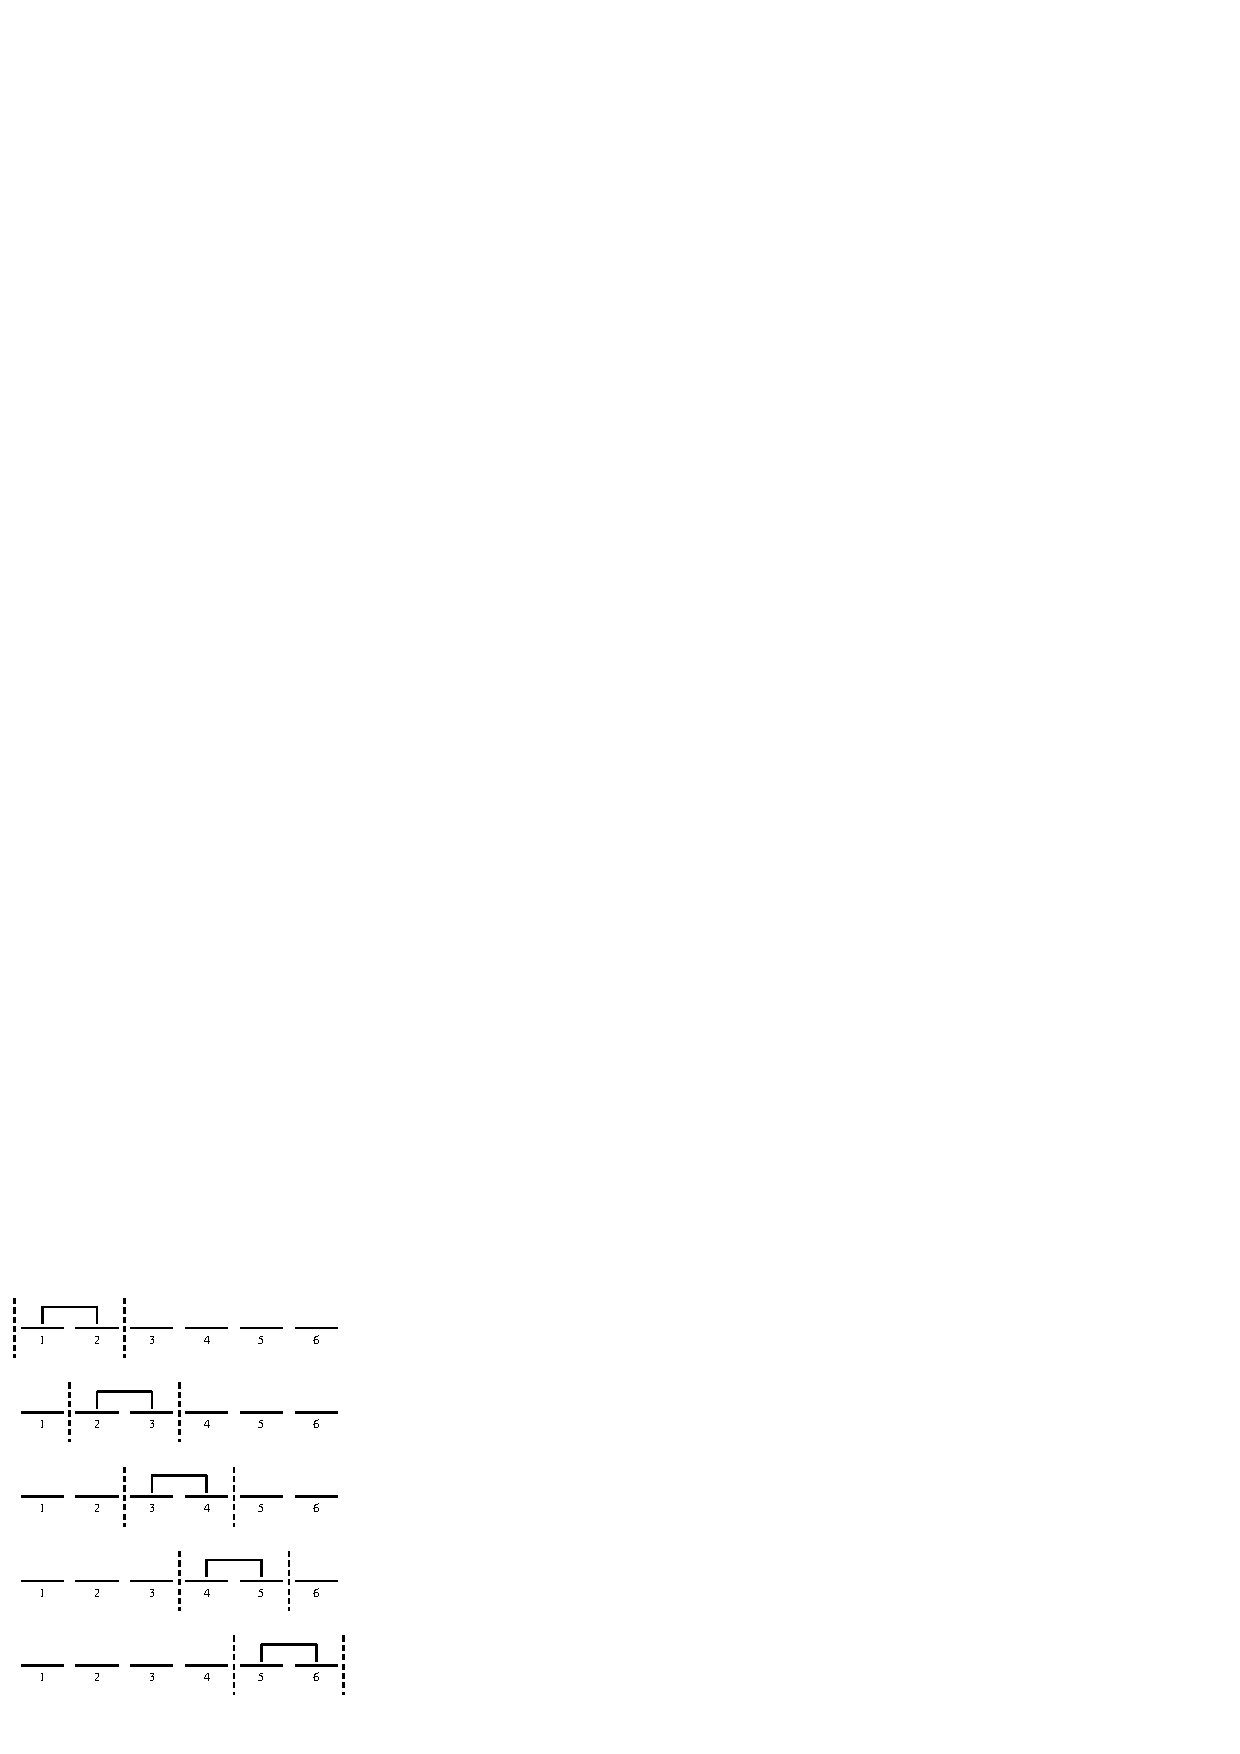
\includegraphics{fig14.pdf}
\captionof{figure}{\emph{Un parking linéaire de $6$ tirets avec une voiture garée sur des places successives}.}
\end{center}

Ainsi, nous pouvons facilement calculer le nombre moyen de voitures qui se garent sur un parking linéaire de $6$ tirets. En effet, telle la méthode appliquée au cas où : $t=4$, il nous suffit de faire la moyenne du nombre moyen de voitures qui segarent sur chaque sous-parkings.

Donc, dans le $1^{er}$ sous-parking, nous avons en moyenne : $1+\operatorname{L}\left(4\right)$ voitures qui se garent soit :
\[1+\frac{5}{3}=\frac{8}{3}\text{ voitures.}\]

Dans le second sous-parking nous avons en moyenne :
\[1+\operatorname{L}\left(3\right)=2\text{ voitures.}\]

Dans le troisième sous-parking c'est assez simple, il y a en moyenne $3$ voitures (la parking est donc saturé). Et nous finissons (grâce à la symétrie) que dans le quatrième et le cinquième sous-parking le nombre moyen de voitures garées est, respectivement, le même que pour les sous-parkings $(2)$ et $(1)$. Ainsi, nous pouvons enfin faire notre moyenne :
\[\operatorname{L}\left(6\right)=\frac{1}{5}\left(\frac{8}{3}+2+3+2+\frac{8}{3}\right)=\frac{1}{5}\left(2\times\frac{8}{3}+2\times2+3\right)=\frac{1}{15}\left(16+12+9\right)=\frac{37}{15}\]

Ainsi, finalement, le nombre moyen de voitures qui se garent sur $6$ tirets que de $\frac{37}{15}$. 

Or, en prêtant un peu plus attention à la décomposition en sous-parkings, nous pouvons remarquer qu'à chaque découpage, $2$ parkings sont crées (même dans le $1^{er}$ sous-parkings avec $0$ tiret à gauche de la voiture garée). Nous établissons donc la définition suivante :

\newDef{\emph{Le nombre moyen de voitures qui se garent sur $t$ tirets correspond à la moyenne du nombre moyen de voitures qui se garent sur chacun de ses sous-parkings}.}

Et puisque à chaque nouveau sous-parking crée, la voiture se déplace de $1$ tiret vers la droite, il découle que le parking à gauche croît de $1$ tiret par nouveau sous-parking contrairement au petit parking de droite qui lui, décroît à la même allure. Et ainsi, nous établissons formellement la formule de récurrence:
\[\operatorname{L}\left(t\right)=\frac{1}{t-1}\sum_{k=0}^{t-2}1+\operatorname{L}\left(k\right) + \operatorname{L}\left(t-2-k\right),\text{ avec : $t\geqslant2$}\]

En effet, puisqu'il y a $t-1$ places sur un parking linéaire de $t$ tirets\footnote{En effet, soit un parking linéaire de $t$ tirets. Soit $t$ est pair soit impair. Si il est pair, le parking peut être rempli, il y a alors $\frac{t}{2}$ voitures garée et décaler chaque voiture de $1$ tiret mène à $\frac{t}{2}+\frac{t}{2}-1=t-1$ places disponibles (la voiture au bout est éjectée). De même lorsque $t$ est impair sauf que la voiture au bout n'est pas éjectée.}, lorsqu'on effectue la moyenne on retrouve bien le $t-1$ au dénominateur. Idem, puisqu'il y a une voiture qui se déplace d'un bout à l'autre du parking, le nombre de tirets à gauche croît de $0$ à $t-2$ et celui de droite décroît de $t-2$ à $0$, ce qui justifie bien la formule générale de récurrence trouvée. 

Notez que le $1$ à l'intérieur du signe \emph{sigma} correspond à la voiture déjà garée sur chacun des sous-parkings.

Finalement, dans la suite du paragraphe, nous allons améliorer notre formule grâce à deux astuces.
\subsubsection{Simplifications \& améliorations par la symétrie}
Dans cette seconde partie, nous allons simplifier notre formule de récurrence qui était :
\[\operatorname{L}\left(t\right)=\frac{1}{t-1}\sum_{k=0}^{t-2}1+\operatorname{L}\left(k\right) + \operatorname{L}\left(t-2-k\right),\text{ avec : $t\geqslant2$}\]

Déjà, à première vu, nous pouvons extraire du signe sigma le $1$. En effet, puisqu'il nous allons faire $t-1$ itérations (n'oublions pas le $0$ !), il suite que : $1\times\left(t-1\right)=t-1$ et donc, nous avons :
\[\operatorname{L}\left(t\right)=\frac{1}{t-1}\sum_{k=0}^{t-2}1+\operatorname{L}\left(k\right) + \operatorname{L}\left(t-2-k\right)=1+\frac{1}{t-1}\sum_{k=0}^{t-2}\operatorname{L}\left(k\right) + \operatorname{L}\left(t-2-k\right),\text{ avec : $t\geqslant2$}\]

Car après avoir tout sommé, il faut diviser par $t-1$ et ainsi $\frac{t-1}{t-1}=1$. 

Mais lorsque nous analysons plus en profondeur les deux termes à l'intérieur du signe \emph{sigma}, on voit que le terme $\operatorname{L}\left(t-2-k\right)$ est très... hideux. Mais nous pouvons tourner la situation à notre avantage ! En effet le terme peut être supprimé assez aisément par la symétrie. 

Lorsque nous décomposons un parking linéaire en sous-parkings nous remarquons la chose suivante (avec ici, un parking linéaire de $6$ tirets) :
\begin{center}
\includegraphics{fig15.pdf}
\captionof{figure}{\emph{Un parking linéaire de $6$ tirets avec une voiture garée sur des places successives}.}
\end{center}

Nous remarquons donc que les deux termes : $\operatorname{L}\left(k\right)$ et $\operatorname{L}\left(t-2-k\right)$ prennent tous les deux les mêmes valeurs, mais pas successivement. Donc, en résumant les valeurs prises par ces deux termes dans un tableau nous obtenons :
\begin{center}
\begin{tabular}{|c||c|c|}
    \hline
    \multicolumn{3}{|c|}{\textbf{Tableau des valeurs de $\operatorname{L}\left(k\right)$ et de $\operatorname{L}\left(t-2-k\right)$ pour $t=6$}} \\ \hline\hline
        \multirow{1}{*}{\emph{$k$}} & \emph{Valeur de $\operatorname{L}\left(k\right)$} & \emph{Valeur de $\operatorname{L}\left(4-k\right)$} \\ \hline\hline
        \multirow{1}{*}{$0$} & $0$ & $\frac{5}{3}$ \\ \hline
        \multirow{1}{*}{$1$} & $0$ & $1$ \\ \hline
        \multirow{1}{*}{$2$} & $1$ & $1$ \\ \hline
        \multirow{1}{*}{$3$} & $1$ & $0$ \\ \hline
        \multirow{1}{*}{$4$} & $\frac{5}{3}$ & $0$ \\
    \hline
\end{tabular}
\captionof{figure}{\emph{Tableau des valeurs successives de $\operatorname{L}\left(k\right)$ et de $\operatorname{L}\left(t-2-k\right)$}.}
\end{center}

Et ainsi, nous pouvons remarquer la chose suivante :
\[(\text{I})\ \ \ \ \sum_{k=0}^{t-2}\operatorname{L}\left(t-2-k\right)=\sum_{k=0}^{t-2}\operatorname{L}\left(k\right)\]

Autrement dit en reprenant la précédente formule de $\operatorname{L}\left(t\right)$ nous avons l'égalité suivante :
\[\operatorname{L}\left(t\right)=1+\frac{1}{t-1}\sum_{k=0}^{t-2}\operatorname{L}\left(k\right) + \operatorname{L}\left(t-2-k\right)=1+\frac{2}{t-1}\sum_{k=0}^{t-2}\operatorname{L}\left(k\right),\text{ avec : $t\geqslant2$}\]

Car la somme générale (à gauche) peut se découper en deux autre sommes plus petite. Et en appliquant l'égalité $(\text{I})$ nous obtenons deux sommes égales, d'où l'apparition du $2$ au numérateur.

Ainsi, nous avons trouvé une formule de récurrence plus courte que la première. Mais il demeure un énorme désavantage avec ces deux formules. En effet, elles disent que pour calculer $\operatorname{L}\left(t\right)$ il est nécessaire d'utiliser toutes les valeurs $\operatorname{L}\left(k\right)$ pour $k\leqslant t-2$. Et par conséquent, l'ordinateur étant limité en stockage de données ainsi qu'en puissance, le calcul de $\operatorname{L}\left(t\right)$ pour de grandes valeurs de $n$ demeure long et coûteux, tant en puissance qu'en mémoire...

C'est pourquoi dans la prochaine partie nous allons trouver une nouvelle formule de récurrence pour calculer $\operatorname{L}\left(t\right)$, mais cette fois-ci en utilisant seulement les deux valeurs qui la précèdent, autrement dit, en utilisant : $\operatorname{L}\left(t-2\right)$ et $\operatorname{L}\left(t-1\right)$. Pas mal non ?
\subsubsection{Une formule de récurrence à l'ordre $2$}
Dans cette partie nous allons améliorer les formules précédentes afin d'obtenir une formule de récurrence seulement d'ordre $2$, c'est-à-dire, qui ne nécessite que les deux termes précédents pour calculer le terme suivant.

Nous savons que nous avions les deux égalités suivantes :
\[\left(\text{I}\right)\ \ \ \ \operatorname{L}\left(t\right)=1+\frac{2}{t-1}\sum_{k=0}^{t-2}\operatorname{L}\left(k\right),\text{ avec : $t\geqslant2$, et}\]
\[\left(\text{II}\right)\ \ \ \ \operatorname{L}\left(t+1\right)=1+\frac{2}{t}\sum_{k=0}^{t-1}\operatorname{L}\left(k\right),\text{ avec : $t\geqslant1$}\]

Mais nous avons immédiatement remarqué à quel point ces deux égalités sont très proches. En effet, les seules distinctions ont lieu au dénominateur de la fraction ainsi qu'à la somme qui s'arrête à $t-2$ dans l'égalité $\left(\text{I}\right)$ contre $t-1$ dans la suivante. 

Or nous savons que :
\[\frac{1}{t}=\frac{t-1}{t}\times\frac{1}{t-1}=\left(1-\frac{1}{t}\right)\times\frac{1}{t-1}\]

Ainsi, en multipliant l'égalité $\left(\text{I}\right)$ par $\left(1-\frac{1}{t}\right)$ nous obtenons :
\[\left(1-\frac{1}{t}\right)\times\operatorname{L}\left(t\right)=\left(1-\frac{1}{t}\right)+\frac{2}{t}\sum_{k=0}^{t-2}\operatorname{L}\left(k\right),\text{ avec : $t\geqslant2$}\]

Et finalement, en ajoutant $\frac{1}{t}$ de part et d'autre afin d'annuler le terme $-\frac{1}{t}$ présent à droite, nous obtenons une égalité très proche de $\operatorname{L}\left(t+1\right)$. Le fait est qu'il ne manque plus qu'à ajouter aussi de part et d'autre le terme $\frac{2}{t}\times\operatorname{L}\left(t-1\right)$ afin de remplacer le $t-2$ du signe \emph{sigma} par un $t-1$. Finalement, nous obtenons :
\[\left(1-\frac{1}{t}\right)\times\operatorname{L}\left(t\right)+\frac{2}{t}\times\operatorname{L}\left(t-1\right)+\frac{1}{t}=1+\frac{2}{t}\sum_{k=0}^{t-1}\operatorname{L}\left(k\right)=\operatorname{L}\left(t+1\right),\text{ avec : $t\geqslant1$}\]

Ainsi nous avons notre fameuse relation de récurrence à l'ordre $2$ qui est la suivante :
\[\operatorname{L}\left(t+1\right)=\left(1-\frac{1}{t}\right)\operatorname{L}\left(t\right)+\frac{2}{t}\operatorname{L}\left(t-1\right)+\frac{1}{t},\text{ avec : $t\geqslant1$}\]

Nous remarquons que cette nouvelle relation est beaucoup plus attrayante que les deux précédentes, d'une part par sa simplicité (pas de signe \emph{sigma} à perte de vu) et d'autre part, par le peu de calculs à fournir. En effet, cette nouvelle formule n'est dépendante que de seulement deux valeurs de la fonction contre presque toutes pour les deux autres formules.

Enfin, dans le paragraphe suivant, nous présenterons les résultats obtenus avec ces deux catégories de formules pour des valeurs de $t$ plus ou moins grandes, avec aussi en prime, le temps mis par l'ordinateur pour les calculer.
\subsection{Résultats obtenus \& imprécisions numériques}
Dans ce paragraphe nous débattrons des résultats procurés par les trois formules trouvées (nous omettrons volontairement ceux données par la première afin de mieux mettre en évidence les deux dernières formules). 

Premièrement, nous construirons un tableau indiquant pour un nombre de tirets croissant les valeurs fournies ainsi que le temps de calculs de la machine. Notez aussi que les deux programmes seront affichés (même si cela n'est pas vraiment nécessaire).
\subsubsection{Les formules \emph{brutes}}
Dans cette partie nous allons montrer quelques résultats obtenus à l'aide de la formule de récurrence ci-dessous :
\[\left(\text{I}\right)\ \ \ \ \operatorname{L}\left(t\right)=1+\frac{2}{t-1}\sum_{k=0}^{t-2}\operatorname{L}\left(k\right),\text{ avec : $t\geqslant2$}\]

Mais avant de commencer à montrer les résultats ordonnées dans un tableau avec le temps de calcul, nous allons montrer le programme qui se cache derrière ceci. Voici le programme en Python :
\begin{center}
\begin{minted}[bgcolor=bg, linenos, frame=single, framesep=12pt]{python}
l1=[0,0] # Nombre moyen de voiture en fonction du nombre de tirets.
def E_1(t):
    if len(l1)>=t+1:return l1[t]        # On test si la valeur existe.
    else:                               # Sinon, on la calcule.
        s=0
        for i in range(t-1):s+=l1[i]    # On somme.
        l1.append(1+2*s/(t-1))          # On peaufine la sommation.
        return l1[-1]                   # On retourne le résultat obtenu.
\end{minted}
\captionof{figure}{\emph{Le code source du programme Python (formule $1$)}.}
\end{center}

Il reste néanmoins relativement simple car il s'agit de mettre en œuvre une petite récursion classique. La liste permet d'éviter de calculer toutes les autres valeurs précédentes évitant de saturer la machine et de perdre du temps... \emph{précieux}.

Ainsi, nous résumons ci-dessous dans un tableaux les calculs qui ont été effectués :
\begin{center}
\begin{tabular}{|c||c|c|}
    \hline
    \multicolumn{3}{|c|}{\textbf{Tableau des valeurs de $\operatorname{L}\left(t\right)$ pour $t$ croissant}} \\ \hline\hline
        \multirow{1}{*}{\emph{$t$}} & \emph{Valeur de $\operatorname{L}\left(t\right)$ (approximation)} & \emph{Temps de calcul en $s$ (approximation)} \\ \hline\hline
        \multirow{1}{*}{$10$} & $4{,}18800705467372$ & $2\cdot10^{-4}\ s$ \\ \hline
        \multirow{1}{*}{$50$} & $21{,}4812826358481$ & $2{,}5\cdot10^{-3}\ s$ \\ \hline
        \multirow{1}{*}{$100$} & $43{,}0979005549328$ & $1\cdot10^{-2}\ s$ \\ \hline
        \multirow{1}{*}{$500$} & $216{,}030843907611$ & $2{,}5\cdot10^{-1}\ s$ \\ \hline
        \multirow{1}{*}{$1000$} & $432{,}197023098458$ & $9\cdot10^{-1}\ s$ \\ \hline
        \multirow{1}{*}{$1500$} & $648{,}363202289305$ & $2\ s$ \\ \hline
        \multirow{1}{*}{$2000$} & $864{,}529381480154$ & $3{,}5\ s$ \\ \hline
        \multirow{1}{*}{$2500$} & $1080{,}695560671$ & $5{,}4\ s$ \\ \hline
        \multirow{1}{*}{$3000$} & $1296{,}86173986185$ & $7{,}8\ s$ \\ \hline
        \multirow{1}{*}{$3500$} & $1513{,}0279190527$ & $10{,}4\ s$ \\ \hline
        \multirow{1}{*}{$4000$} & $1729{,}19409824354$ & $14{,}3\ s$ \\ \hline
        \multirow{1}{*}{$4026$} & $1740{,}43473956147$ & $15\ s$ \\
    \hline
\end{tabular}
\captionof{figure}{\emph{Tableau des valeurs de $\operatorname{L}\left(t\right)$ pour un nombre $t$ de tirets croissant}.}
\end{center}

Ainsi, au vu du tableau ci-dessus, nous voyons bien que plus le nombre de tirets augmente, plus le temps de calcul se rallonge jusqu'à atteindre les $15$ secondes pour obtenir une approximation de la réponde au problème $\operatorname{L}\left(4026\right)$. Mais $15$ secondes paraît un temps bien long par rapport à celui que donnera la prochaine formule de récurrence.

Ainsi, grâce à cette formule nous avons enfin obtenu la réponde à notre problème :
\[\operatorname{L}\left(4026\right)=\lambda_L\approx 1740{,}43473956147\]

Ce qui semble coïncider avec le résultat trouvé par l'ordinateur dans la section précédente qui était d'environ :
\[\operatorname{L}\left(4026\right)=\lambda_L\approx1740{,}4354741\]

Remarquez la précision de celui-ci : $2$ décimales exactes ! Alors qu'on ne connaissait même pas la formule de récurrence (le taux d'erreur n'est seulement que de $\epsilon = 0{,}0007345385299686313$ !). Mais le gros problème de cette formule arrive lorsque nous souhaitons calculer précisément le résultat sous forme d'une fraction, le temps de calcul devient alors phénoménale (en effet, la machine doit stocker des fractions de plus en plus grandes, il doit toutes les additionner et ainsi de suite...).

Finalement, nous allons passer à le seconde formule de récurrence (à l'ordre $2$) qui promet d'être bien plus rapide.
\subsubsection{La formule de récurrence à l'ordre $2$}
Dans cette seconde partie, nous montrerons les résultats obtenus grâce à la formule de récurrence à l'ordre $2$. Nous effectuerons les mêmes calculs et nous comparerons (dans la partie suivante) à l'aide d'un graphique le temps de calcul en fonction du nombre de tirets. Cette fois-ci, la formule de récurrence utilisée est celle-ci :
\[\operatorname{L}\left(t+1\right)=\left(1-\frac{1}{t}\right)\operatorname{L}\left(t\right)+\frac{2}{t}\operatorname{L}\left(t-1\right)+\frac{1}{t},\text{ avec : $t\geqslant1$}\]

Mais, comme pour la partie précédente, nous allons d'abord afficher le code source de la fonction permettant d'effectuer les calculs (il s'agit de l'implémentation, en Python de la formule de récurrence ci-dessus) :
\begin{center}
\begin{minted}[bgcolor=bg, linenos, frame=single, framesep=12pt]{python}
l2=[0,0] # Nombre moyen de voiture en fonction du nombre de tirets.
def E_2(t):
    global l2                     # Ceci permet de modifier la liste l2.
    # On calcule et on ajoute dans la liste la valeur suivante.
    l2.append((t-2)*l2[1]+2*l2[0]+1)/(t-1)) 
    l2=l2[1:]                     # On supprime la plus vieille.
\end{minted}
\captionof{figure}{\emph{Le code source du programme Python (formule $2$)}.}
\end{center}

Ce programme est assez similaire au programme précédent. Mais néanmoins, il paraît beaucoup plus simple. En effet, même si nous utilisons encore le système de la liste, celle-ci contient toujours le même nombre d'éléments, et ainsi, ne surcharge pas la mémoire de l'ordinateur. De plus, nous n'avons pas besoin de sommer tous les éléments de la liste. Ainsi, la formule de récurrence à l'ordre $2$ donne les résultats suivant, classés dans un tableau :
\begin{center}
\begin{tabular}{|c||c|c|}
    \hline
    \multicolumn{3}{|c|}{\textbf{Tableau des valeurs de $\operatorname{L}\left(t\right)$ pour $t$ croissant}} \\ \hline\hline
        \multirow{1}{*}{\emph{$t$}} & \emph{Valeur de $\operatorname{L}\left(t\right)$ (approximation)} & \emph{Temps de calcul en $s$ (approximation)} \\ \hline\hline
        \multirow{1}{*}{$10$} & $4{,}18800705467372$ & $2\cdot10^{-4}\ s$ \\ \hline
        \multirow{1}{*}{$50$} & $21{,}4812826358481$ & $8\cdot10^{-4}\ s$ \\ \hline
        \multirow{1}{*}{$100$} & $43{,}0979005549328$ & $1\cdot10^{-3}\ s$ \\ \hline
        \multirow{1}{*}{$500$} & $216{,}030843907611$ & $8{,}2\cdot10^{-3}\ s$ \\ \hline
        \multirow{1}{*}{$1000$} & $432{,}197023098457$ & $1{,}7\cdot10^{-2}\ s$ \\ \hline
        \multirow{1}{*}{$1500$} & $648{,}363202289303$ & $2{,}5\cdot10^{-2}\ s$ \\ \hline
        \multirow{1}{*}{$2000$} & $864{,}529381480151$ & $3{,}5\cdot10^{-2}\ s$ \\ \hline
        \multirow{1}{*}{$2500$} & $1080{,}695560671$ & $4{,}2\cdot10^{-2}\ s$ \\ \hline
        \multirow{1}{*}{$3000$} & $1296{,}86173986184$ & $5{,}4\cdot10^{-2}\ s$ \\ \hline
        \multirow{1}{*}{$3500$} & $1513{,}02791905269$ & $6\cdot10^{-2}\ s$ \\ \hline
        \multirow{1}{*}{$4000$} & $1729{,}19409824354$ & $7\cdot10^{-2}\ s$ \\ \hline
        \multirow{1}{*}{$4026$} & $1740{,}43473956146$ & $7\cdot10^{-2}\ s$ \\
    \hline
\end{tabular}
\captionof{figure}{\emph{Tableau des valeurs de $\operatorname{L}\left(t\right)$ pour un nombre $t$ de tirets croissant}.}
\end{center}

Même remarque que pour la formule précédente, le temps de calcul augmente lorsque le nombre $t$ de tirets croît. Mais ici, nous remarquons plusieurs choses. D'une part, le temps de calcul ne dépasse même pas le dixième de seconde (ce qui est très rapide) ! C'est pour cela que la formule de récurrence à l'ordre $2$ est beaucoup plus performante pour faire des calculs sur le long terme. 

Or, si nous regardons plus précisément les résultats trouvés par ces deux formules, nous pouvons voir que les dernières décimales ne sont pas toujours identiques. Parfois l'une va mettre un $8$ contre un $7$, un $7$ contre un $69$ et ainsi de suite...

Mais c'est cette accumulation d'erreurs qui conduit, pour $t$ suffisamment grand, à des calculs erronés. Enfin, néanmoins, nous obtenons un résultat assez proche de celui obtenu avec la formule précédente pour $t=4026$. En effet, on a :
\[\operatorname{L}\left(4026\right)=\lambda_L\approx1740{,}43473956146\footnote{Notez que le résultats n'est valable qu'uniquement pour un parking linéaire de $4026$ tirets. Si nous voulons $\operatorname{C}\left(4026\right)$ il suffit d'appliquer la relation entre les fonctions $\operatorname{C}$ et $\operatorname{L}$, autrement dit : $\operatorname{C}\left(4026\right)=1+\operatorname{L}\left(4024\right)=\lambda_C\approx1+1739{,}5700748447=1740{,}5700748447$. Les deux résultats sont légèrement différents mais cela n'a pas vraiment d'importance...}\]

De plus, cette formule permet de calculer le nombre moyen de voitures pour un nombre $t$ de tirets très grand, ainsi, voici un graphique avec les valeurs de $\operatorname{L}\left(t\right)$ avec $0\leqslant t\leqslant5\cdot10^6$ :

\begin{center}
\includegraphics[scale=0.5]{../Graphiques/Graphique_Moyenne.png}
\captionof{figure}{\emph{Graphique des $5$ premières millions de valeurs de $\operatorname{L}$ pour $0\leqslant n\leqslant 5\ 000\ 000$}.}
\end{center}

Nous remarquons immédiatement que cette fonction semble avoir un comportement proportionnelle. Qui sait ?

Cette formule possède un avantage majeur : elle permet de calculer le résultat le plus précis qui soit. En effet, avec l'aide du module \emph{fractions}, Python peut calculer un résultat sous forme d'une fraction. C'est ce que nous avons fait avec la formule de récurrence à l'ordre $2$. Mais la fractions est... trop grande\footnote{Si par curiosité vous voudriez voir les résultats $\lambda_L$ et $\lambda_C$ jetez un coup d'œil dans le dossier \emph{Solutions 4026}.} ! Finalement, nous allons comparer les performances des deux formules dans la partie qui suit.
\subsubsection{Performance : comparaison des deux formules de récurrence}
Dans cette partie, nous allons comparer les performances des deux formules avec plusieurs graphiques. Premièrement, un graphique montrant la vitesse de calcul en fonction du nombre de tirets. Puis, deux autres visant à montrer la vitesse des deux programmes, l'un par rapport à l'autre. Voici le premier graphique :

\begin{center}
\includegraphics[scale=0.5]{../Graphiques/Comparaison/2_formules/Comparaison_1.png}
\captionof{figure}{\emph{Graphique de la vitesse de calcul des deux programmes $P_1$ (formule $1$) et $P_2$ (formule $2$)}.}
\end{center}

Nous remarquons que la courbe bleue ($1^{ère}$ formule) croît très rapidement alors la seconde croît, très lentement (rappelons qu'elle ne dépasse même pas le dixième de seconde !). Mais maintenant, nous allons comparer les vitesses de calcul, autrement dit, combien de fois le programme $2$ (respectivement $1$) peut être exécuté afin qu'il mette le même temps que le premier programme (respectivement, le second). Voici pour commencer le programme indiquant les différentes valeurs du quotient, $\frac{P_1}{P_2}$ :

\begin{center}
\includegraphics[scale=0.5]{../Graphiques/Comparaison/Formule_1_2/VitesseCalcul_1_2.png}
\captionof{figure}{\emph{Comparaison du programme $P_1$ par rapport à $P_2$ (voir les tableaux ci-dessus)}.}
\end{center}

Nous voyons que la courbe croît très vite ce qui est normal puisque d'après les deux tableaux plus haut, le premier programme atteint les $15$ secondes alors que le premier n'a même pas dépasser le dixième de seconde. On pourrait résumé ce graphique de la manière suivante : \emph{Combien de fois faudrait-il exécuter le programme $P_2$ pour que le temps de calcul de celui-ci s'équilibre avec une seule exécution du programme $P_1$ ?} Maintenant nous faisons de même mais avec les valeurs du quotient $\frac{P_2}{P_1}$ :

\begin{center}
\includegraphics[scale=0.5]{../Graphiques/Comparaison/Formule_2_1/VitesseCalcul_2_1.png}
\captionof{figure}{\emph{Comparaison du programme $P_2$ par rapport à $P_1$ (voir les tableaux ci-dessus)}.}
\end{center}

Et ici, contrairement au graphique ci-dessus, la courbe décroît très vite. Ce qui est aussi normal au vu des deux tableaux étudiés. De même, on pourrait résumé ce graphique de la manière suivante : \emph{Combien de fois faudrait-il exécuter le programme $P_1$ pour que le temps de calcul de celui-ci s'équilibre avec une seule exécution du programme $P_2$ ?} 

Ainsi, nous avons finalement résolut le problème du parking. 

$\claim$

\end{document}
